%inizio capitolo 2
\chapter{Algoritmo di gestione dinamica applicato ad un singolo incrocio \label{capitolo2}}

In questo capitolo si vuole analizzare il comportamento dello stesso incrocio visto in precedenza con un algoritmo di gestione ottimizzata, che conti il numero di auto in ciascuna corsia e in base a questo e ad altri parametri conceda il verde per un numero di secondi variabile. È da precisare che l’algoritmo utilizzato si basa su quello proposto da \textit{Maram Bani Younes e Azzedine Boukerche}\cite{itlc}, tuttavia sono state effettuate alcune importanti modifiche, che verranno analizzate nel corso della trattazione. 

Si è previsto,  oltre che un raffronto fra l'algoritmo di gestione statica e quello sviluppato in autonomia, modificando quanto proposto dai due ingegneri, anche un meccanismo per valutare l'efficacia di queste modifiche, confrontando il nuovo codice con una implementazione di quello presente nella pubblicazione citata. Tutti i confronti, con i relativi grafici e le relative conclusioni, verranno presentati alla fine di questo capitolo, dopo aver descritto nel dettaglio tutti gli aspetti relativi alle modifiche apportate al modello e ai meccanismi implementativi adottati.


Per quanto riguarda lo pseudocodice progettato dai due ingegneri, è disponibile alla seguente pagina.
\newpage
\begin{lstlisting}[language=C,label=pseudocode,caption=Pseudocodice di gestione dinamica di un incrocio]
while d_i di una qualsiasi corsia > 0 do
{
	
	sia j la corsia con il maggior numero di macchine;
	siano i_1 e i_2 le due corsie complementari;
		if (d_i_1 > d_i_2)
		{
			schedula j,i_1;
			d_i_1 = 0;
			t_i_1 = 0;
		}
		
		else
		{
			schedula j,i_2;
			d_i_2 = 0;
			t_i_2 = 0;
		}
		d_j = 0;
		t_j = 0;
	
}   
\end{lstlisting}
\newpage
\section{Breve spiegazione dell'algoritmo originale}
La proposta di \textit{Maram Bani Younes e Azzedine Boukerche} si basa sulla definizione di alcuni parametri, il primo dei quali è la così detta \textit{Ready Area}. Tale area è sostanzialmente il range entro il quale le macchine si possono considerare in coda per l’incrocio: si individua, per ogni semaforo della giunzione, una distanza massima, di solito corrispondente alla portata del dispositivo di rilevazione in termini di veicoli, oltre la quale le vetture non vengono più conteggiate. 

Il dispositivo in questione può essere rappresentato da una semplice telecamera che, mediante meccanismi tipici della Computer Vision, utilizzando API quali Google Vision\cite{google_vision} o OpenCV\cite{open_CV}, riesca ad individuare la variabile principale su cui si basa l’algoritmo: il numero di auto in coda per ciascuna corsia. L’implementazione hardware di questo sistema, tuttavia, non è oggetto di questa tesi e dunque non ci si dilungherà oltre nella sua spiegazione.

Il tempo concesso alle corsie prescelte (durata della luce verde) è poi dinamico, e viene calcolato sulla base della seguente formula: 

\begin{equation} \label{eq:}
  T = \theta + \frac{F_d}{S_{tf}}
\end{equation}

Il parametro $\theta$ è una costante, e rappresenta il tempo che mediamente è necessario alla prima macchina per partire, mentre $F_d$ è la distanza del veicolo più lontano dal semaforo (sempre interno alla \textit{Ready Area} ). In ultimo, $S_{tf}$ è la velocità media del flusso di auto nell’intersezione. Come è ovvio notare, sia $\theta$ che $S_{tf}$ sono ottenuti mediante delle stime, non essendo misurabili prima della effettiva esecuzione dell’algoritmo. 

Una proposta alternativa, certamente più efficiente ma anche meno facile da implementare, è quella di permettere alle automobili di comunicare fra loro e con il semaforo dati quali la $F_d$ (distanza), nonché la loro velocità media. Certamente in questo modo si renderebbe l’esecuzione dello script più veritiera ed affidabile, ed in futuro, grazie agli sforzi delle case automobilistiche, probabilmente tutto ciò sarà possibile.

Altri parametri da considerare sono $d_i$ che rappresenta il numero di automobili in coda nella corsia i-esima e $t_i$, tempo richiesto a tutti i veicoli della corsia i-esima (all’interno della \textit{Ready Area}) per lasciare l’intersezione.

\textbf{Il funzionamento dell’algoritmo è dunque il seguente:} si individua la corsia più affollata fra quella che presentano almeno un’automobile, e contestualmente si rintracciano le due corsie compatibili con essa, così come spiegato nel \textit{Capitolo \ref{capitolo1}} e come si può notare nella \textit{figura \ref{dirCompatibili}}.

A questo punto, fra queste due candidate si sceglie ancora la più affollata; in questo modo non solo si va a concedere il verde alla strada con più automobili, ma si cerca anche di ottimizzare la scelta della sua complementare, che non resta statica (come invece è nell’algoritmo utilizzato nel capitolo precedente), ma diventa dinamica ed intelligente. Successivamente l’algoritmo prevede di calcolare il tempo \textit{T}, concedendolo alla luce verde delle due corsie, e di azzerare le variabili $d_i, d_j$ e $t_i, t_j$ relative, in quanto si prevede che dopo T secondi le corsie in questione presentino un numero di veicoli pari a zero.
\newpage
\section{Le modifiche apportate}
Sono molteplici le modifiche apportate all’algoritmo proposto, alcune delle quali a puro scopo implementativo, altre come migliorie.

In primo luogo, si è preferito non considerare una \textit{Ready Area} per non dover dare alle code di \textit{Simulink} un massimo numero di entità (veicoli) da contenere, questo per effettuare più simulazioni variando i tassi di generazione, verificando il comportamento del modello anche in condizioni esageratamente negative, con code anche molto affollate (più di 50 automobili). 

Il concetto della \textit{Ready Area}, tuttavia, non è stato abbandonato del tutto, ma è stato piuttosto migliorato: si è deciso di concedere un tempo minimo ed un tempo massimo alla durata del verde per ciascuna corsia. Il tempo minimo serve perché, anche con una sola macchina in coda, si è voluto stabilizzare la situazione, che altrimenti si sarebbe tradotta in un passaggio troppo repentino dal verde al rosso. Per quanto concerne il tempo massimo, questo è diretta espressione della \textit{Ready Area}: invece che considerare un massimo numero di veicoli, si considera che, indipendentemente da questo numero, il verde non può durare più di un certo valore, questo per evitare tempi di attesa troppo lunghi nelle corsie meno affollate, ma comunque in cui sono presenti veicoli. 

Il tempo concesso alla luce verde, poi, viene calcolato tenendo conto della distribuzione uniforme che governa gli \textit{Entity Server}, precedentemente descritta, assegnando ad ogni macchina un valore pari al valore medio della distribuzione (in questa simulazione pari a $5s$), ed ottenendo il tempo complessivo moltiplicando questo valore per il numero di veicoli in coda. A questo punto, se il numero ottenuto è inferiore al tempo minimo, esso si scarta, e si prende in considerazione proprio quel minimo, viceversa se supera il tempo massimo è questo ad essere tenuto in considerazione e ad essere concesso. Pertanto, poiché non è detto che le code a cui viene dato il via libera si svuotino, non si va ad azzerare i contatori relativi, ma semplicemente all'esecuzione successiva della funzione questi sono aggiornati con i nuovi dati rilevati, ottenuti dalle code stesse.

Inoltre, è stata individuata una grande lacuna nell’algoritmo oggetto della pubblicazione citata: l’assenza di un meccanismo di gestione della \textit{starvation}. 

Considerando esclusivamente il \textit{codice \ref{pseudocode}}, infatti, si nota che se in una strada continuano a confluire veicoli più velocemente che nelle altre, a questa sarà sempre concesso il verde. Questo comportamento da un lato è positivo perché si va a decongestionare tale corsia, ma è ovviamente improponibile, in quanto potrebbe paradossalmente capitare che un semaforo resti rosso per ore ed ore, e che una persona sia costretta ad attendere un tempo esagerato prima di passare, perché la sua strada è meno affollata.

È stato scelto dunque di implementare un meccanismo di gestione della \textit{starvation} mediante un algoritmo \textit{LRU} (Least Recently Used) opportunamente modificato. Ad ogni corsia è associato un contatore, ed ogni qual volta ad una strada viene concesso il verde, il suo contatore viene azzerato, mentre quello delle altre si incrementa del numero di secondi per cui è stato concesso il verde alla corsia suddetta. In questo modo, quando un contatore raggiunge un valore limite (liberamente impostabile), la relativa strada ottiene priorità massima, e l’algoritmo viene applicato in maniera identica (calcolo del tempo del verde e selezione della complementare) come se essa fosse quella più affollata. In particolare il tempo massimo di attesa prima che scatti la \textit{starvation} è stato impostato a 2.5 minuti.

È anche da notare che sono stati apportati alcuni minimi cambiamenti al modello: le code sono state collegate agli ingressi del blocco contenente la funzione da eseguire, comunicando ad essa il numero di veicoli presenti, inserendo delle \textbf{Input Port \cite{inputport}} nel blocco Function Call Subsystem, ed il canale di \textit{feedback} è stato utilizzato per implementare il meccanismo della gestione della \textit{starvation}, e non per conoscere a quale semaforo è stato concesso il verde nell’esecuzione precedente, informazione ora inutile. Non è stato variato altro, se non, ovviamente, il codice nel blocco \textit{Matlab Function}, quindi non si ravvisa la necessità di descrivere nei dettagli nuovamente l'intero modello, il cui schema è comunque presente alla pagina seguente, seguito dal codice che lo governa.
\newline
\begin{figure}[H]
\centering
  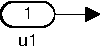
\includegraphics[width=0.25\textwidth]{InputPort.pdf}
  \caption{Input Port}
  \label{fig:inputport}
\end{figure}

\begin{figure}[H]
  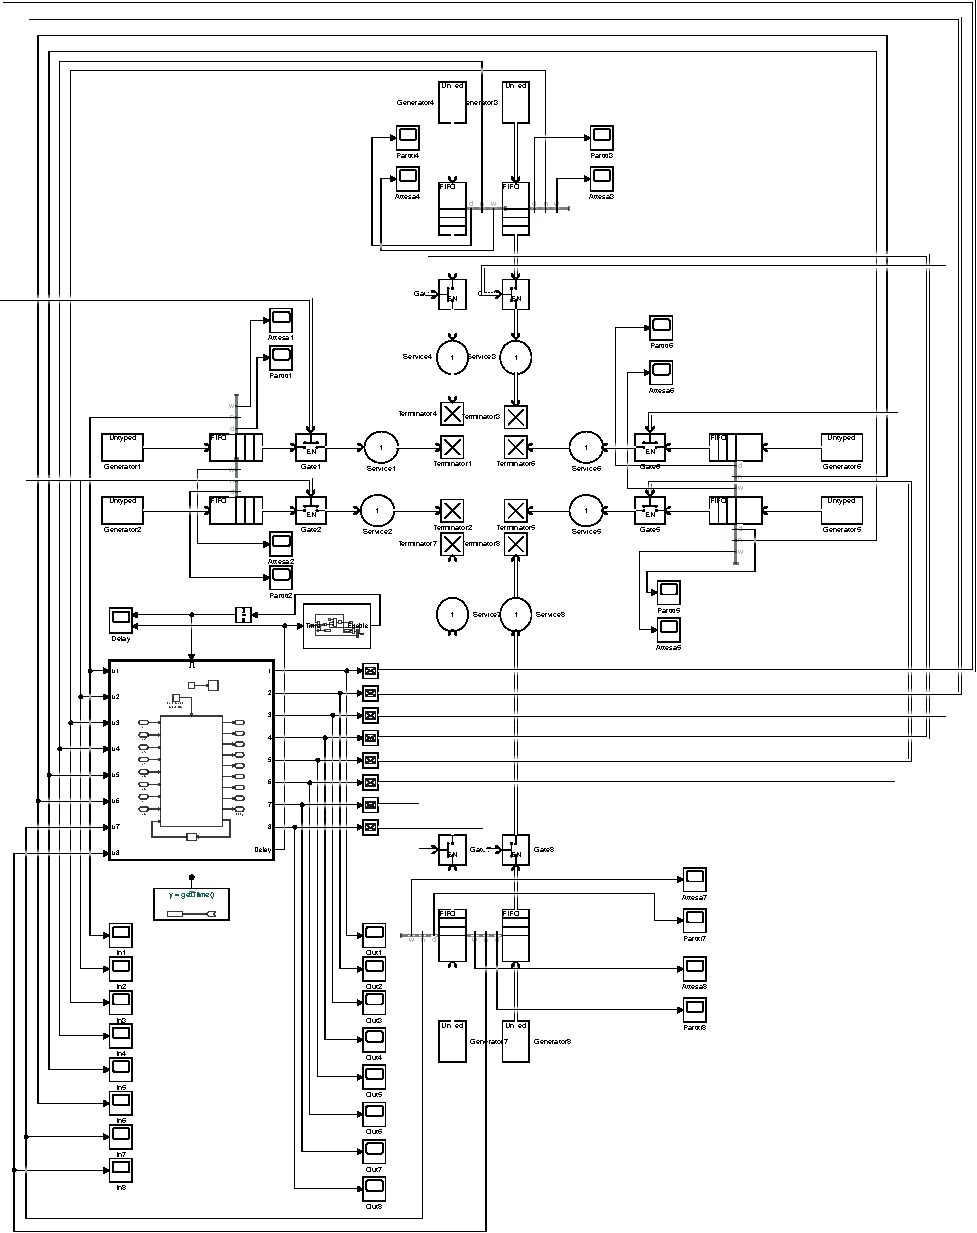
\includegraphics[width=1\textwidth]{SingoloIncrocioAlgoritmo.pdf}
  \caption{Modello di un incrocio a raso a quattro bracci in Simulink e SimEvents, gestione dinamica}
  \label{fig:modellosingoloincrocioalgoritmo}
\end{figure}
\newpage

\begin{lstlisting}[language=Matlab,label=algoritmodin,caption=Implementazione dell'algoritmo di gestione dinamica di un singolo incrocio]
function [delay, y1, y2, y3, y4, y5, y6, y7, y8, feedback] = fcn(u1, u2, u3, u4, u5, u6, u7, u8, history)


% VARIABILI DI USCITA
% Prima attesa, prima dell'esecuzione dell'algoritmo la prima volta
delay = 1; 
y1 = 0; 
y2 = 0; 
y3 = 0; 
y4 = 0; 
y5 = 0; 
y6 = 0; 
y7 = 0;
y8 = 0;
feedback = zeros([4 2]);
 
% Numero di veicoli per ogni direzione
M = ([u1 u2; u3 u4; u5 u6; u7 u8;]);
 
% Tempo medio per fluire per ogni macchina
Tv = 5;
 
% Massimo tempo del verde
MaxGreen = 35;
 
% Minimo tempo del verde
MinGreen = 15;
 
% Controllo sulla starvation (LRU). Tempo di attesa massimo: 2.5 minuti
starvation = 150;
 
% Cerco il massimo
[R, C] = size(M);
iMax = 1;
jMax = 1;
vMax = M(1, 1);
 
%Usato per la starvation, interrompe la ricerca
flag = 0;
 
for i = 1 : 1 : R
    for j = 1 : 1 : C
        
        if M(i, j) > 0 && history(i, j) > starvation
            vMax = M(i, j);
            iMax = i;
            jMax = j;
            flag = 1;
            break;
        end
 
        if M(i, j) > vMax
            vMax = M(i, j);
            iMax = i;
            jMax = j;
        end
       
    end
    
    if flag == 1
        break;
    end
end
 
 
% Cerco i possibili candidati
[c1_i, c1_j, c2_i, c2_j] = getCandidates(iMax, jMax);
 
%Scelgo tra i candidati
if M(c1_i, c1_j) > M(c2_i, c2_j) 
    iCan = c1_i;
    jCan = c1_j;
else
    iCan = c2_i;
    jCan = c2_j;
end
 
delay = vMax*Tv;
 
if vMax*Tv > MaxGreen
        delay = MaxGreen;
elseif vMax*Tv < MinGreen
        delay = MinGreen;
end
    
%Risultato
U = ([0 0; 0 0; 0 0; 0 0]);
 
U(iMax, jMax) = 1;
U(iCan, jCan) = 1;
     
history( : ) = history( : ) + delay;
    
history(iMax, jMax) = 0;
history(iCan, jCan) = 0;

%Output 
y1 = U(1, 1); y2 = U(1, 2); y3 = U(2, 1); y4 = U(2, 2); y5 = U(3, 1); y6 = U(3, 2); y7 = U(4, 1); y8 = U(4, 2); feedback(:) = history(:);
end
    
\end{lstlisting}
\newpage
\section{Spiegazione del codice implementato}
In primo luogo vengono inizializzate le variabili in uscita della funzione, corrispondenti al valore di trigger degli otto entity gate rappresentanti i vari semafori. Di default questi valori sono posti a 0 (semaforo rosso). In input si accetta il numero di veicoli presenti in ogni coda nell'istante in cui la funzione viene richiamata, nonché il vettore \textit{history}, usato per gestire la \textit{starvation}, il cui significato sarà chiaro più avanti.

I due \textit{cicli for} annidati servono ad individuare la strada con il numero di veicoli più elevato, purché non si verifichi il caso di \textit{starvation}. Tale strada (individuata da due indici, \textit{i} e \textit{j} all’interno della matrice \textit{M}, matrice che organizza gli otto input indipendenti), viene poi data in pasto alla funzione \textit{getCandidates}, il cui codice è alla pagina seguente e che restituisce gli indici relativi alla matrice M che individuano le due strade che possono essere scelte assieme alla principale. A questo punto fra le due corsie complementari candidate viene scelta, come già detto, quella più affollata. Viene calcolato il tempo da concedere al verde in funzione del numero di veicoli della strada scelta come principale, e vengono effettuati i controlli con il tempo minimo ed il tempo massimo, precedentemente dichiarati come costanti.

Successivamente, ogni elemento del vettore \textit{History}, il quale contiene i contatori inerenti all’algoritmo \textit{LRU} per ogni corsia, viene incrementato del tempo stabilito, azzerando poi gli elementi corrispondenti alle corsie a cui si sta concedendo il verde.

In output viene inviato \textit{1} agli \textit{Entity Gate} che devono aprirsi, corrispondenti alle strade individuate, e \textit{0} a tutti gli altri. 

Oltre a queste informazioni rappresenta un output anche il \textit{delay}, ovvero proprio il tempo concesso, che viene inviato al timer descritto nel \textit{capitolo \ref{capitolo1}}, che richiamerà la funzione allo scadere dello stesso.

La matrice M è stata creata seguendo la struttura della seguente tabella, ritenuta agevole per l'implementazione dell'algoritmo.
\newline
\begin{table}[H]
\centering
\begin{tabular}{|c|c|c|}
  \hline
  & 
  \textbf{Colonna 1} & 
  \textbf{Colonna 2} \\\hline
  Riga 1 & 
  Corsia Ovest - Sinistra & 
  Corsia Ovest - Dritto/Destra \\\hline
  Riga 2 & 
  Corsia Nord - Sinistra & 
  Corsia Nord - Dritto/Destra \\\hline
  Riga 3 & 
  Corsia Est - Sinistra & 
  Corsia Est - Dritto/Destra \\\hline
  Riga 4 & 
  Corsia Sud - Sinistra & 
  Corsia Sud - Dritto/Destra \\\hline
\end{tabular}
\caption{Matrice della lunghezza delle code per ogni corsia}
\label{table:matrix-length-corsia}
\end{table}

\newpage
\begin{lstlisting}[language=Matlab,label=key,caption=Scelta delle due strade complementari a quella selezionata come principale]
    function [i1, j1, i2, j2] = getCandidates(i, j)
    % Direzioni accoppiate (8x4)
    % Per ciascuna direzione scelta, ci sono 2 possibili direzioni
    % complementari
    % D = {[1 2; 3 1] [1 1; 3 2]; [4 1; 2 2] [2 1; 4 2]; [3 2; 1 1] [3 1; 1 2]; [4 2; 2 1] [4 1; 2 2]};
    
    i1 = 0;
    i2 = 0;
    j1 = 0;
    j2 = 0;
    
    if i==1 && j ==1
        i1 = 1;
        j1 = 2;
        i2 = 3;
        j2 = 1;
    elseif i==1 && j==2
       i1 = 1;
       j1 = 1;
       i2 = 3;
       j2 = 2;
    elseif i==2 && j==1
       i1 = 4;
       j1 = 1;
       i2 = 2;
       j2 = 2;
    elseif i==2 && j==2
       i1 = 2;
       j1 = 1;
       i2 = 4;
       j2 = 2;
    elseif i==3 && j==1
       i1 = 3;
       j1 = 2;
       i2 = 1;
       j2 = 1;
    elseif i==3 && j==2
       i1 = 3;
       j1 = 1;
       i2 = 1;
       j2 = 2;
    elseif i==4 && j==1
       i1 = 4;
       j1 = 2;
       i2 = 2;
       j2 = 1;
    elseif i==4 && j==2
       i1 = 4;
       j1 = 1;
       i2 = 2;
       j2 = 2;
    end
            
        
end
\end{lstlisting}

È da sottolineare che questo codice funziona fintanto che gli ingressi non vengono variati: se si dovesse collegare una strada ad un ingresso diverso da quello previsto ed utilizzato nella simulazione chiaramente l’intero algoritmo non sarebbe più affidabile. L'autore di questa tesi è consapevole che esistono metodi più eleganti ed ottimizzati rispetto a questa sequenza di \textit{if} ed \textit{elseif} per ottenere il medesimo scopo, tuttavia si è reso necessario procedere in questo modo per lo scarso supporto del linguaggio \textit{Matlab} a tali meccanismi, come, per esempio, gli \textit{switch - case}. In questo modo, inoltre, il codice risulta particolarmente leggibile e facile da comprendere.
\newline

Le differenze con un normale algoritmo di gestione di una giunzione, come quello proposto nel \textit{capitolo \ref{capitolo1}} sono quindi evidenti: in primo luogo non si segue una turnazione statica per quanto riguarda la concessione del verde, seguendo invece un meccanismo di priorità: ci si chiede infatti quale sia la strada che necessita del verde in quell'istante, più delle altre, e glielo si concede. Inoltre anche il tempo per cui questo verde è concesso è variabile: si ipotizzi per esempio di analizzare l'incrocio durante le ore notturne, non avrebbe senso concedere il verde per un numero di secondi elevato quando in coda è presente una sola macchina: si tratterebbe di una perdita di tempo, tradotta in un maggior consumo di carburante ed un maggiore stress per gli automobilisti delle altre corsie, costretti ad attendere perché viene concesso il verde ad una strada praticamente vuota. Viceversa è ovvio che durante il giorno, per una strada affollata, la durata della luce verde deve essere sufficiente da garantire che un buon numero delle macchine in coda defluisca.
\newpage

\section{Il modello per confrontare le diverse gestioni del singolo incrocio}

I benefici esposti, ovviamente, devono trovare riscontro in un confronto imparziale ed assolutamente valido fra i modelli presentati, affinché a partire dai medesimi dati in input (le automobili generate), e con gli stessi parametri (tasso di generazione, tempo di servizio interno agli \textit{Entity Server}) essi gestiscano l'incrocio secondo la propria logica. Si è scelto, pertanto, di creare in un nuovo workspace il modello identificato dalla \textit{figura \ref{fig:gatecontrolcompare}}. Si può notare come al suo interno siano presenti tre blocchi principali, ognuno dei quali è rappresentativo di un algoritmo di gestione. Guardando infatti ai tre blocchi presenti, si comprende subito come questi siano in realtà esattamente i modelli precedentemente descritti. Il primo, quello più in alto a sinistra, è quello presentato nel \textit{capitolo \ref{capitolo1}}, relativo ad una gestione statica (\textit{figura \ref{fig: modelloSingoloIncrocio}}). Quello in basso a sinistra invece si riferisce al modello di controllo dinamico, di cui si è parlato in questo capitolo (\textit{figura \ref{fig:modellosingoloincrocioalgoritmo}}), mentre quello in basso a destra è perfettamente identico a quest'ultimo, eccezion fatta per la gestione della \textit{starvation}, che si è eliminata. Ciò è stato fatto per capire come tale gestione, che comunque resta assolutamente necessaria, interferisca con il normale funzionamento dell'algoritmo stesso.

Nello specifico, in questo terzo modello, si è provveduto semplicemente a commentare la seguente porzione di codice, lasciando tutto il resto invariato.
\newline
\begin{lstlisting}[language=Matlab,label=starvation,caption= Porzione di codice relativa alla gestione della starvation]
    if M(i, j) > 0 && history(i, j) > starvation
            vMax = M(i, j);
            iMax = i;
            jMax = j;
            flag = 1;
            break;
    end
        ...
        ...
        ...
   if flag == 1
        break;
   end
\end{lstlisting}

Gli \textit{Entity Generator}, poi, sono stati collegati a dei blocchi di tipo \textbf{Entity Replicator\cite{entityreplicator}}, in modo tale che appena una entità viene generata in una corsia specifica, questa venga subito inviata ai tre modelli contemporaneamente. In questo modo i tre incroci sono esattamente identici sia per quanto riguarda il numero di entità che devono gestire che per quanto concerne quando queste si presentano, tutto questo per garantire l'assoluta imparzialità delle condizioni, precedentemente citata. Il Replicator è stato configurato seguendo lo schema in figura.
\newline

\begin{figure}[H]
\centering
  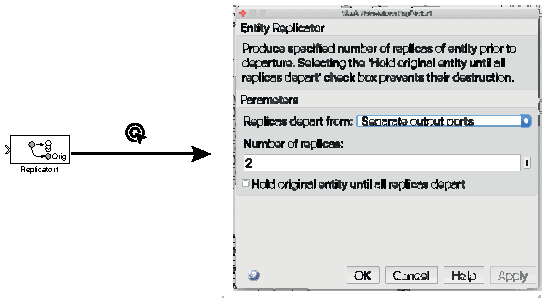
\includegraphics[width=1\textwidth]{replicatorEProprieta.pdf}
  \caption{Entity Replicator e relative proprietà}
  \label{fig:}
\end{figure}

Dunque il workflow è il seguente: quando una entità viene generata, questa viene inviata a tutti e tre gli incroci, in corrispondenza della stessa corsia e nello stesso istante di tempo. La simulazione parte allo stesso istante per tutti e tutti sono configurati secondo gli stessi parametri. Al termine della simulazione tutti gli incroci producono tre grafici per ogni corsia, relativi al tempo di attesa medio, al numero di macchine totali che hanno attraversato tale strada ed al numero di macchine in coda in funzione dell'ora del giorno. Confrontando i grafici di una stessa strada, e facendo questo per ogni strada presente, si ottiene una chiara idea di quale dei tre algoritmi stia funzionando meglio.

\newpage

\begin{figure}[H]
  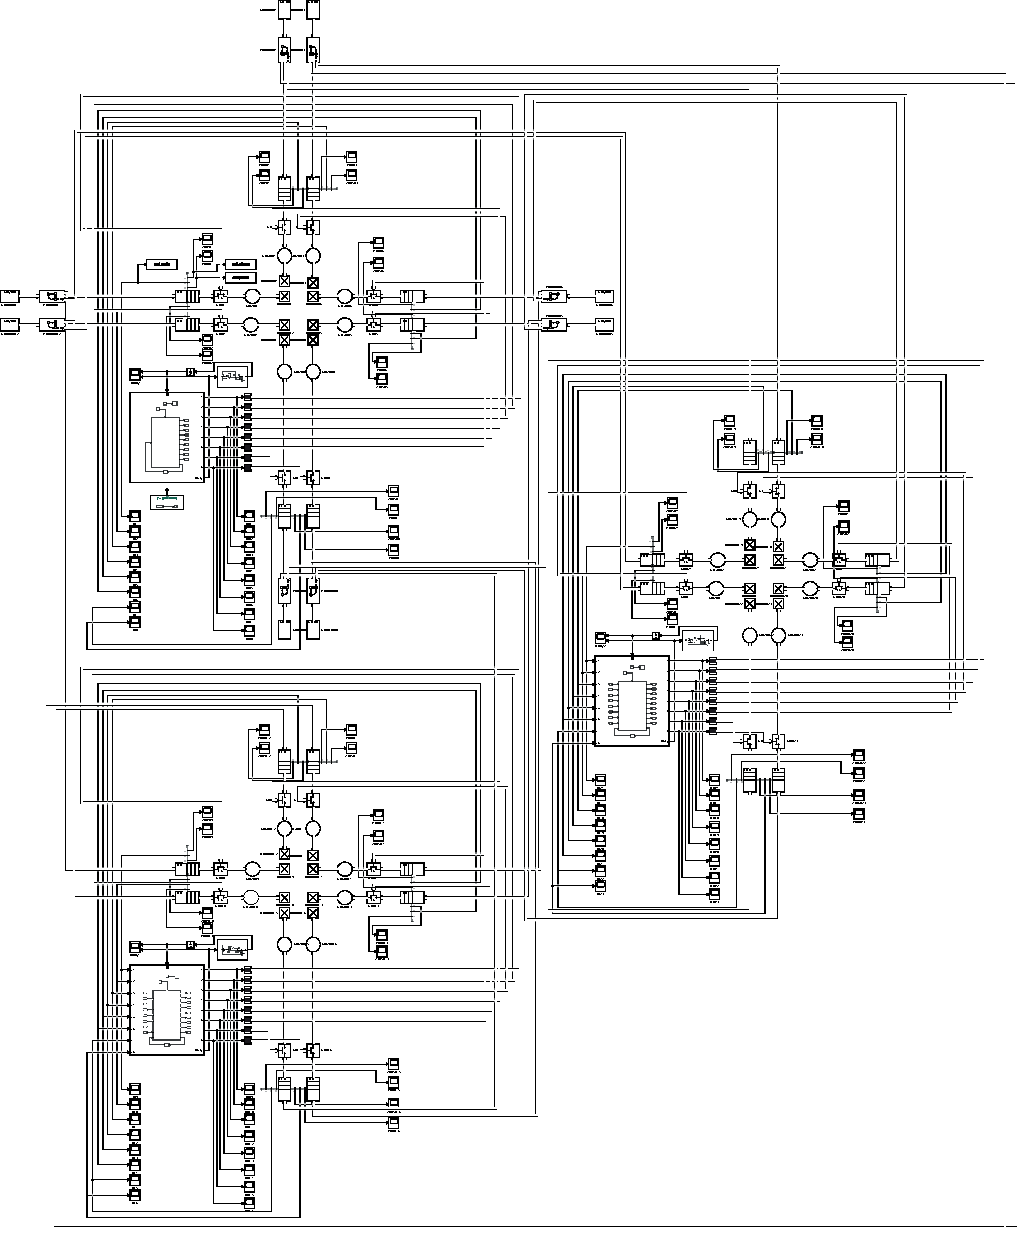
\includegraphics[width=1\textwidth]{GateControlCompare.pdf}
  \caption{Modello per comparare gli algoritmi utilizzati per la gestione di un singolo incrocio}
  \label{fig:gatecontrolcompare}
\end{figure}

\newpage
\section{I risultati ottenuti}
Per le seguenti simulazioni il primo scenario, ovvero il seguente, presenta dei tassi di generazione randomici, esattamente come nel \textit{capitolo \ref{capitolo1}}, con il parametro $\mu$ scelto casualmente, secondo una distribuzione uniforme, fra 23 e 35 ed un tempo di servizio pari a $5s$, rispetto ad un numero randomico fra $4s$ e $6s$ come spiegato in precedenza, per eliminare questa ulteriore variabile casuale. Questo per ottenere un numero di automobili sì variabile, ma che sia confrontabile fra le varie strade, con una configurazione dunque che può dirsi bilanciata. Il codice interno agli \textit{Entity Generator} non è dunque stato variato rispetto a quanto presentato nel \textit{codice \ref{mu-definition}}, così come la definizione dei parametri globali (\textit{codice \ref{entity-generator}}).

Il tempo di concessione massima del verde, poi, è stato impostato a $35s$, e quello minimo a $15s$, come si può notare nel codice presentato precedentemente.

In una configurazione di questo genere sono stati ottenuti i risultati riportati nelle seguenti tabelle.
\newline

\begin{table}[H]
\centering
\begin{tabular}{|C{2cm}|C{1.65cm}|C{1.65cm}|C{1.65cm}|C{1.65cm}|C{1.65cm}|C{1.65cm}|}
  \hline
  \multicolumn{7}{|c|}{\large Prima simulazione: prime quattro corsie} \\\hline\hline
  \textbf{Intervallo} &
  \multicolumn{3}{C{5.8cm}|}{\textbf{Stima tempo interarrivo con minimo $\mu$}} &
  \multicolumn{3}{C{5.8cm}|}{\textbf{Stima tempo interarrivo con massimo $\mu$}} \\\hline
  $[23, 35]$ &
  \multicolumn{3}{c|}{$15.94s$} &
  \multicolumn{3}{c|}{$24.26$} \\\hline
  \multirow{7}{2cm}{\centering \textit{\footnotesize{Corsia Ovest \newline --- \newline Sinistra}}}
  & \multicolumn{2}{C{3.7cm}|}{\textbf{$\mu$}} 
  & \multicolumn{2}{C{3.7cm}|}{\textbf{\footnotesize{Tempo di arrivo medio}}} 
  & \multicolumn{2}{C{3.7cm}|}{\textbf{\footnotesize{Numero di auto totale}}} \\\cline{2-7}
  & \multicolumn{2}{C{3.7cm}|}{24.1705} 
  & \multicolumn{2}{C{3.7cm}|}{$16.75s$} 
  & \multicolumn{2}{C{3.7cm}|}{2940} \\\cline{2-7}
  & \multicolumn{2}{C{3.7cm}|}{\footnotesize{\textbf{Gestione statica}}} 
  & \multicolumn{2}{C{3.7cm}|}{\footnotesize{\textbf{Gestione dinamica senza starvation}}} 
  & \multicolumn{2}{C{3.7cm}|}{\footnotesize{\textbf{Gestione dinamica con starvation}}} \\\cline{2-7}
  & \scriptsize{Max numero auto in coda}
  & \scriptsize{Tempo di attesa medio}
  & \scriptsize{Max numero auto in coda}
  & \scriptsize{Tempo di attesa medio}
  & \scriptsize{Max numero auto in coda}
  & \scriptsize{Tempo di attesa medio}\\\cline{2-7}
  & 25
  & $59.44s$
  & 11
  & $19.18s$
  & 13
  & $19.07s$\\\hline\hline
    \multirow{7}{2cm}{\centering \textit{\footnotesize{Corsia Ovest \newline --- \newline Dritto/Destra}}}
  & \multicolumn{2}{C{3.7cm}|}{\textbf{$\mu$}} 
  & \multicolumn{2}{C{3.7cm}|}{\textbf{\footnotesize{Tempo di arrivo medio}}} 
  & \multicolumn{2}{C{3.7cm}|}{\textbf{\footnotesize{Numero di auto totale}}} \\\cline{2-7}
  & \multicolumn{2}{C{3.7cm}|}{26.3420} 
  & \multicolumn{2}{C{3.7cm}|}{$18.26s$} 
  & \multicolumn{2}{C{3.7cm}|}{2809} \\\cline{2-7}
  & \multicolumn{2}{C{3.7cm}|}{\footnotesize{\textbf{Gestione statica}}} 
  & \multicolumn{2}{C{3.7cm}|}{\footnotesize{\textbf{Gestione dinamica senza starvation}}} 
  & \multicolumn{2}{C{3.7cm}|}{\footnotesize{\textbf{Gestione dinamica con starvation}}} \\\cline{2-7}
  & \scriptsize{Max numero auto in coda}
  & \scriptsize{Tempo di attesa medio}
  & \scriptsize{Max numero auto in coda}
  & \scriptsize{Tempo di attesa medio}
  & \scriptsize{Max numero auto in coda}
  & \scriptsize{Tempo di attesa medio}\\\cline{2-7}
  & 18
  & $52.61s$
  & 8
  & $17.27s$
  & 10
  & $17.34s$\\\hline\hline
  \multirow{7}{2cm}{\centering \textit{\footnotesize{Corsia Nord \newline --- \newline Sinistra}}}
  & \multicolumn{2}{C{3.7cm}|}{\textbf{$\mu$}} 
  & \multicolumn{2}{C{3.7cm}|}{\textbf{\footnotesize{Tempo di arrivo medio}}} 
  & \multicolumn{2}{C{3.7cm}|}{\textbf{\footnotesize{Numero di auto totale}}} \\\cline{2-7}
  & \multicolumn{2}{C{3.7cm}|}{29.5626} 
  & \multicolumn{2}{C{3.7cm}|}{$20.49s$} 
  & \multicolumn{2}{C{3.7cm}|}{2384} \\\cline{2-7}
  & \multicolumn{2}{C{3.7cm}|}{\footnotesize{\textbf{Gestione statica}}} 
  & \multicolumn{2}{C{3.7cm}|}{\footnotesize{\textbf{Gestione dinamica senza starvation}}} 
  & \multicolumn{2}{C{3.7cm}|}{\footnotesize{\textbf{Gestione dinamica con starvation}}} \\\cline{2-7}
  & \scriptsize{Max numero auto in coda}
  & \scriptsize{Tempo di attesa medio}
  & \scriptsize{Max numero auto in coda}
  & \scriptsize{Tempo di attesa medio}
  & \scriptsize{Max numero auto in coda}
  & \scriptsize{Tempo di attesa medio}\\\cline{2-7}
  & 10
  & $38.86s$
  & 9
  & $24.02s$
  & 10
  & $22.85s$\\\hline\hline
  \multirow{7}{2cm}{\centering \textit{\footnotesize{Corsia Nord \newline --- \newline Dritto/Destra}}}
  & \multicolumn{2}{C{3.7cm}|}{\textbf{$\mu$}} 
  & \multicolumn{2}{C{3.7cm}|}{\textbf{\footnotesize{Tempo di arrivo medio}}} 
  & \multicolumn{2}{C{3.7cm}|}{\textbf{\footnotesize{Numero di auto totale}}} \\\cline{2-7}
  & \multicolumn{2}{C{3.7cm}|}{34.4901} 
  & \multicolumn{2}{C{3.7cm}|}{$23.91s$} 
  & \multicolumn{2}{C{3.7cm}|}{2049} \\\cline{2-7}
  & \multicolumn{2}{C{3.7cm}|}{\footnotesize{\textbf{Gestione statica}}} 
  & \multicolumn{2}{C{3.7cm}|}{\footnotesize{\textbf{Gestione dinamica senza starvation}}} 
  & \multicolumn{2}{C{3.7cm}|}{\footnotesize{\textbf{Gestione dinamica con starvation}}} \\\cline{2-7}
  & \scriptsize{Max numero auto in coda}
  & \scriptsize{Tempo di attesa medio}
  & \scriptsize{Max numero auto in coda}
  & \scriptsize{Tempo di attesa medio}
  & \scriptsize{Max numero auto in coda}
  & \scriptsize{Tempo di attesa medio}\\\cline{2-7}
  & 11
  & $37.12s$
  & 8
  & $21.31s$
  & 7
  & $21.43s$\\\hline
\end{tabular}
\caption{Tabella di comparazione fra algoritmi di gestione del singolo incrocio - prime quattro corsie - $\mu$ casuali}
\label{table:keytable}
\end{table}
\newpage

\begin{table}[H]
\centering
\begin{tabular}{|C{2cm}|C{1.65cm}|C{1.65cm}|C{1.65cm}|C{1.65cm}|C{1.65cm}|C{1.65cm}|}
  \hline
  \multicolumn{7}{|c|}{\large Prima simulazione: ultime quattro corsie} \\\hline\hline
  \textbf{Intervallo} &
  \multicolumn{3}{C{5.8cm}|}{\textbf{Stima tempo interarrivo con minimo $\mu$}} &
  \multicolumn{3}{C{5.8cm}|}{\textbf{Stima tempo interarrivo con massimo $\mu$}} \\\hline
  $[23, 35]$ &
  \multicolumn{3}{c|}{$15.94s$} &
  \multicolumn{3}{c|}{$24.26$} \\\hline
  \multirow{7}{2cm}{\centering \textit{\footnotesize{Corsia Est \newline --- \newline Sinistra}}}
  & \multicolumn{2}{C{3.7cm}|}{\textbf{$\mu$}} 
  & \multicolumn{2}{C{3.7cm}|}{\textbf{\footnotesize{Tempo di arrivo medio}}} 
  & \multicolumn{2}{C{3.7cm}|}{\textbf{\footnotesize{Numero di auto totale}}} \\\cline{2-7}
  & \multicolumn{2}{C{3.7cm}|}{34.5787} 
  & \multicolumn{2}{C{3.7cm}|}{$23.97s$} 
  & \multicolumn{2}{C{3.7cm}|}{2152} \\\cline{2-7}
  & \multicolumn{2}{C{3.7cm}|}{\footnotesize{\textbf{Gestione statica}}} 
  & \multicolumn{2}{C{3.7cm}|}{\footnotesize{\textbf{Gestione dinamica senza starvation}}} 
  & \multicolumn{2}{C{3.7cm}|}{\footnotesize{\textbf{Gestione dinamica con starvation}}} \\\cline{2-7}
  & \scriptsize{Max numero auto in coda}
  & \scriptsize{Tempo di attesa medio}
  & \scriptsize{Max numero auto in coda}
  & \scriptsize{Tempo di attesa medio}
  & \scriptsize{Max numero auto in coda}
  & \scriptsize{Tempo di attesa medio}\\\cline{2-7}
  & 9
  & $36.93s$
  & 7
  & $18.76s$
  & 8
  & $19.08s$\\\hline\hline
    \multirow{7}{2cm}{\centering \textit{\footnotesize{Corsia Est \newline --- \newline Dritto/Destra}}}
  & \multicolumn{2}{C{3.7cm}|}{\textbf{$\mu$}} 
  & \multicolumn{2}{C{3.7cm}|}{\textbf{\footnotesize{Tempo di arrivo medio}}} 
  & \multicolumn{2}{C{3.7cm}|}{\textbf{\footnotesize{Numero di auto totale}}} \\\cline{2-7}
  & \multicolumn{2}{C{3.7cm}|}{24.8914} 
  & \multicolumn{2}{C{3.7cm}|}{$17.25s$} 
  & \multicolumn{2}{C{3.7cm}|}{2928} \\\cline{2-7}
  & \multicolumn{2}{C{3.7cm}|}{\footnotesize{\textbf{Gestione statica}}} 
  & \multicolumn{2}{C{3.7cm}|}{\footnotesize{\textbf{Gestione dinamica senza starvation}}} 
  & \multicolumn{2}{C{3.7cm}|}{\footnotesize{\textbf{Gestione dinamica con starvation}}} \\\cline{2-7}
  & \scriptsize{Max numero auto in coda}
  & \scriptsize{Tempo di attesa medio}
  & \scriptsize{Max numero auto in coda}
  & \scriptsize{Tempo di attesa medio}
  & \scriptsize{Max numero auto in coda}
  & \scriptsize{Tempo di attesa medio}\\\cline{2-7}
  & 32
  & $65.24s$
  & 11
  & $22.33s$
  & 11
  & $22.48s$\\\hline\hline
  \multirow{7}{2cm}{\centering \textit{\footnotesize{Corsia Sud \newline --- \newline Sinistra}}}
  & \multicolumn{2}{C{3.7cm}|}{\textbf{$\mu$}} 
  & \multicolumn{2}{C{3.7cm}|}{\textbf{\footnotesize{Tempo di arrivo medio}}} 
  & \multicolumn{2}{C{3.7cm}|}{\textbf{\footnotesize{Numero di auto totale}}} \\\cline{2-7}
  & \multicolumn{2}{C{3.7cm}|}{34.6471} 
  & \multicolumn{2}{C{3.7cm}|}{$20.02s$} 
  & \multicolumn{2}{C{3.7cm}|}{1996} \\\cline{2-7}
  & \multicolumn{2}{C{3.7cm}|}{\footnotesize{\textbf{Gestione statica}}} 
  & \multicolumn{2}{C{3.7cm}|}{\footnotesize{\textbf{Gestione dinamica senza starvation}}} 
  & \multicolumn{2}{C{3.7cm}|}{\footnotesize{\textbf{Gestione dinamica con starvation}}} \\\cline{2-7}
  & \scriptsize{Max numero auto in coda}
  & \scriptsize{Tempo di attesa medio}
  & \scriptsize{Max numero auto in coda}
  & \scriptsize{Tempo di attesa medio}
  & \scriptsize{Max numero auto in coda}
  & \scriptsize{Tempo di attesa medio}\\\cline{2-7}
  & 11
  & $37.92s$
  & 8
  & $27.96s$
  & 10
  & $27.16s$\\\hline\hline
  \multirow{7}{2cm}{\centering \textit{\footnotesize{Corsia Sud \newline --- \newline Dritto/Destra}}}
  & \multicolumn{2}{C{3.7cm}|}{\textbf{$\mu$}} 
  & \multicolumn{2}{C{3.7cm}|}{\textbf{\footnotesize{Tempo di arrivo medio}}} 
  & \multicolumn{2}{C{3.7cm}|}{\textbf{\footnotesize{Numero di auto totale}}} \\\cline{2-7}
  & \multicolumn{2}{C{3.7cm}|}{34.4860} 
  & \multicolumn{2}{C{3.7cm}|}{$23.90s$} 
  & \multicolumn{2}{C{3.7cm}|}{2175} \\\cline{2-7}
  & \multicolumn{2}{C{3.7cm}|}{\footnotesize{\textbf{Gestione statica}}} 
  & \multicolumn{2}{C{3.7cm}|}{\footnotesize{\textbf{Gestione dinamica senza starvation}}} 
  & \multicolumn{2}{C{3.7cm}|}{\footnotesize{\textbf{Gestione dinamica con starvation}}} \\\cline{2-7}
  & \scriptsize{Max numero auto in coda}
  & \scriptsize{Tempo di attesa medio}
  & \scriptsize{Max numero auto in coda}
  & \scriptsize{Tempo di attesa medio}
  & \scriptsize{Max numero auto in coda}
  & \scriptsize{Tempo di attesa medio}\\\cline{2-7}
  & 10
  & $36.63s$
  & 11
  & $29.44s$
  & 8
  & $27.69s$\\\hline
\end{tabular}
\caption{Tabella di comparazione fra algoritmi di gestione del singolo incrocio - ultime quattro corsie - $\mu$ casuali}
\label{table:keytable}
\end{table}



Sono riportati, inoltre, alcuni grafici indicativi, inerenti ad una singola corsia (sempre la stessa, quella del braccio ovest relativa alla svolta a sinistra), per ciascuno dei tre modelli, che mostrano il tempo medio d'attesa ed il numero di macchine in coda in funzione dell'ora del giorno.
\newline

\textbf{Nota:} sui grafici relativi ai tempi di attesa viene riportata un'attesa stimata secondo una media temporale cumulativa, ovvero istante per istante sono sommati i tempi di attesa di ogni automobile che ha raggiunto l'incrocio attraverso una strada specifica e sono divisi per il numero complessivo di auto della corsia in questione. L'attesa relativa alla gestione della \textit{starvation}, invece, viene calcolata in base al tempo trascorso fra due concessioni consecutive del verde allo stesso semaforo. Risulta chiaro quindi come in realtà la \textit{starvation} intervenga anche se nei grafici che seguono il tempo di attesa medio non raggiunge mai i 2.5 minuti, in quanto sono due valori diversi. Ci si può rendere conto del fatto che sia intervenuta la \textit{starvation} nella configurazione relativa dal fatto che i valori ottenuti si discostino da quelli inerenti alla gestione dinamica senza \textit{starvation}, seppur di poco. Essendo infatti gli input ed i parametri dei due modelli identici, se la \textit{starvation} non fosse intervenuta, anche gli output sarebbero dovuti essere uguali.

\begin{figure}[H]
\centering
  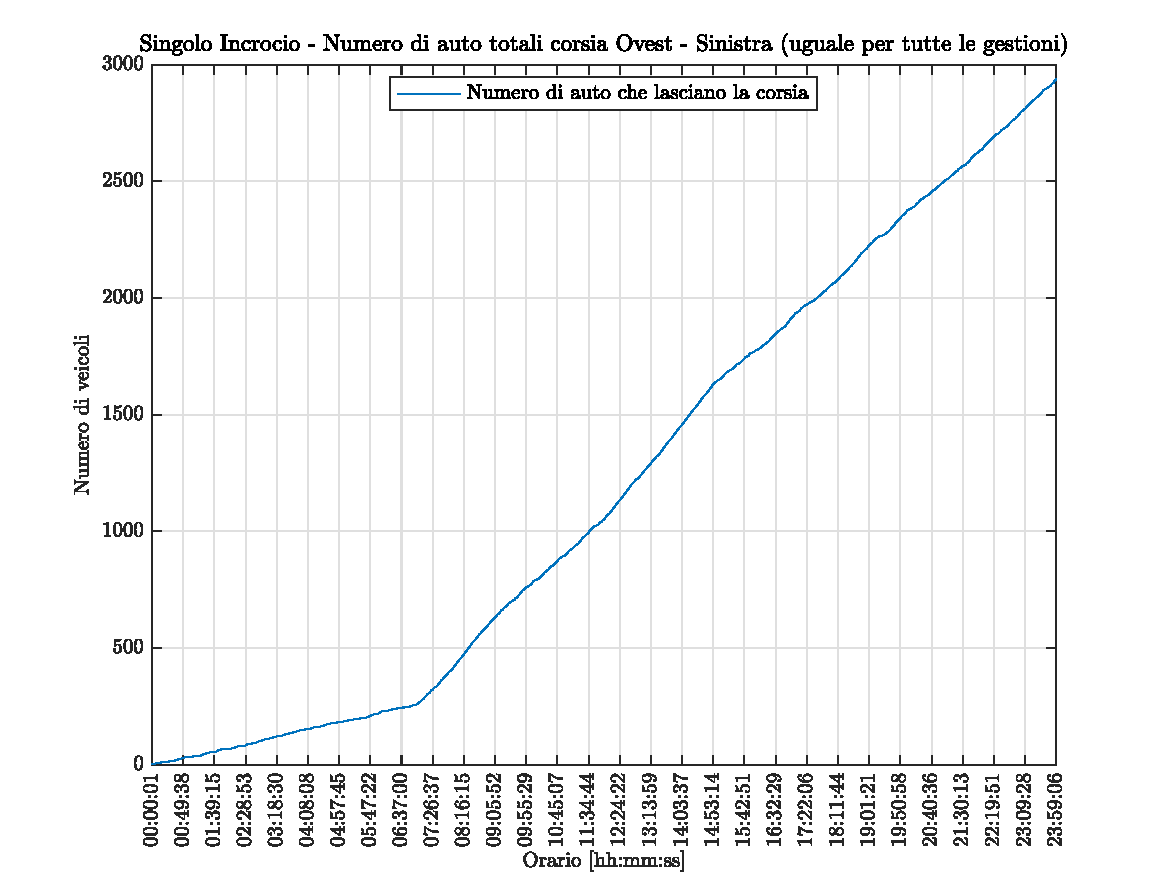
\includegraphics[width=1\textwidth]{figuraPartiti.pdf}
  \caption{Auto che hanno attraversato la corsia Ovest - Sinistra (uguale per i tre modelli di gestione)}
  \label{fig:partitiMuRandom}
\end{figure}

\begin{figure}[H]
\centering
  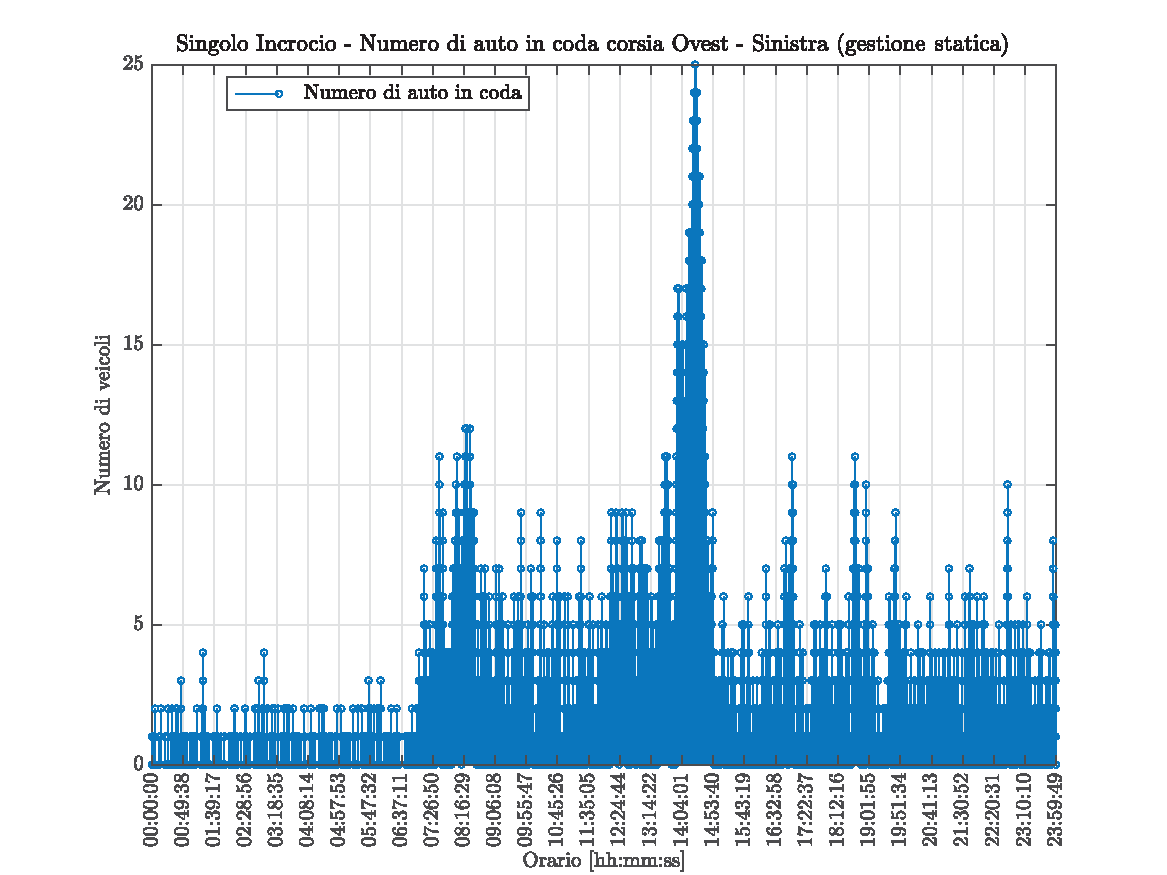
\includegraphics[width=0.9\textwidth]{figuraCodaGestioneStatica.pdf}
  \caption{Numero di auto in coda in funzione dell'ora del giorno - Gestione statica del singolo incrocio - $\mu$ casuali - corsia Ovest - Sinistra}
  \label{fig:}
\end{figure}

\begin{figure}[H]
\centering
  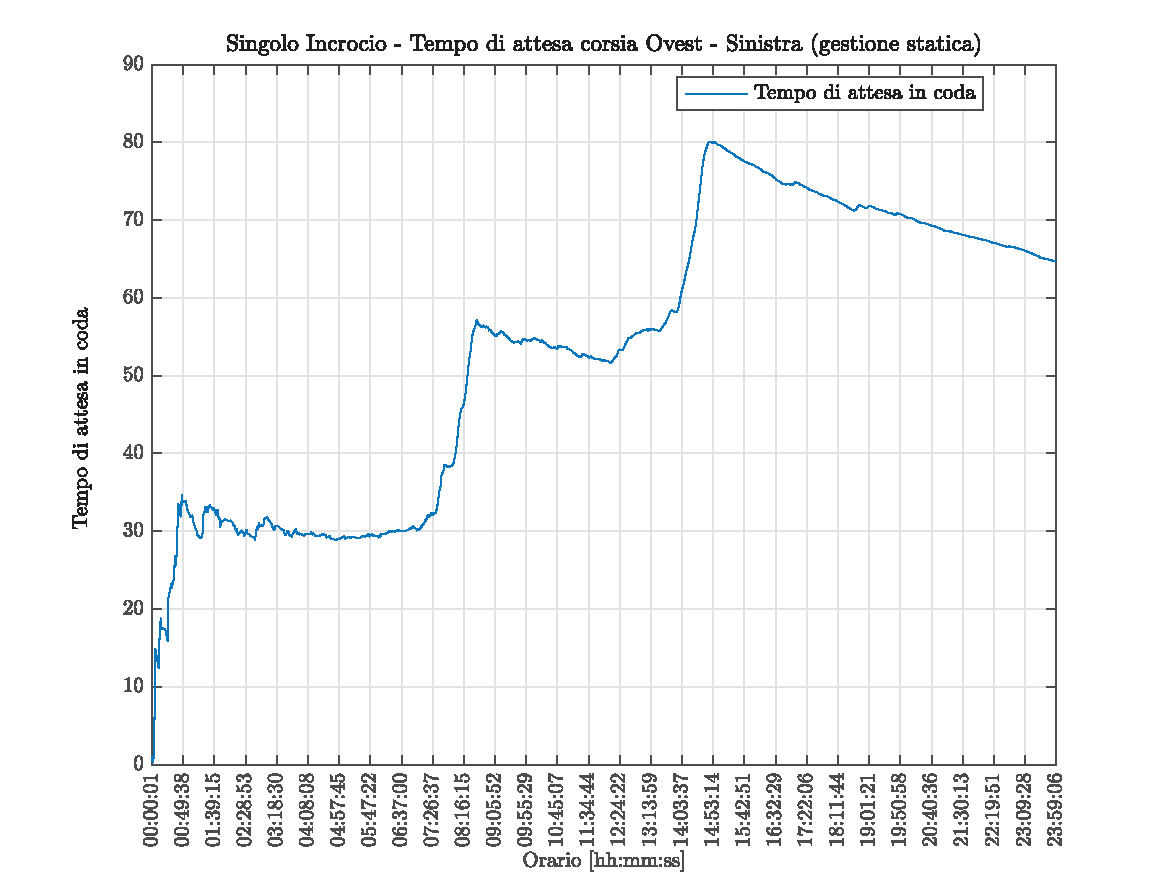
\includegraphics[width=0.9\textwidth]{figuraAttesaGestioneStatica.pdf}
  \caption{Tempi di attesa in funzione dell'ora del giorno - Gestione statica del singolo incrocio - $\mu$ casuali - corsia Ovest - Sinistra}
  \label{fig:}
\end{figure}
\newpage

\begin{figure}[H]
\centering
  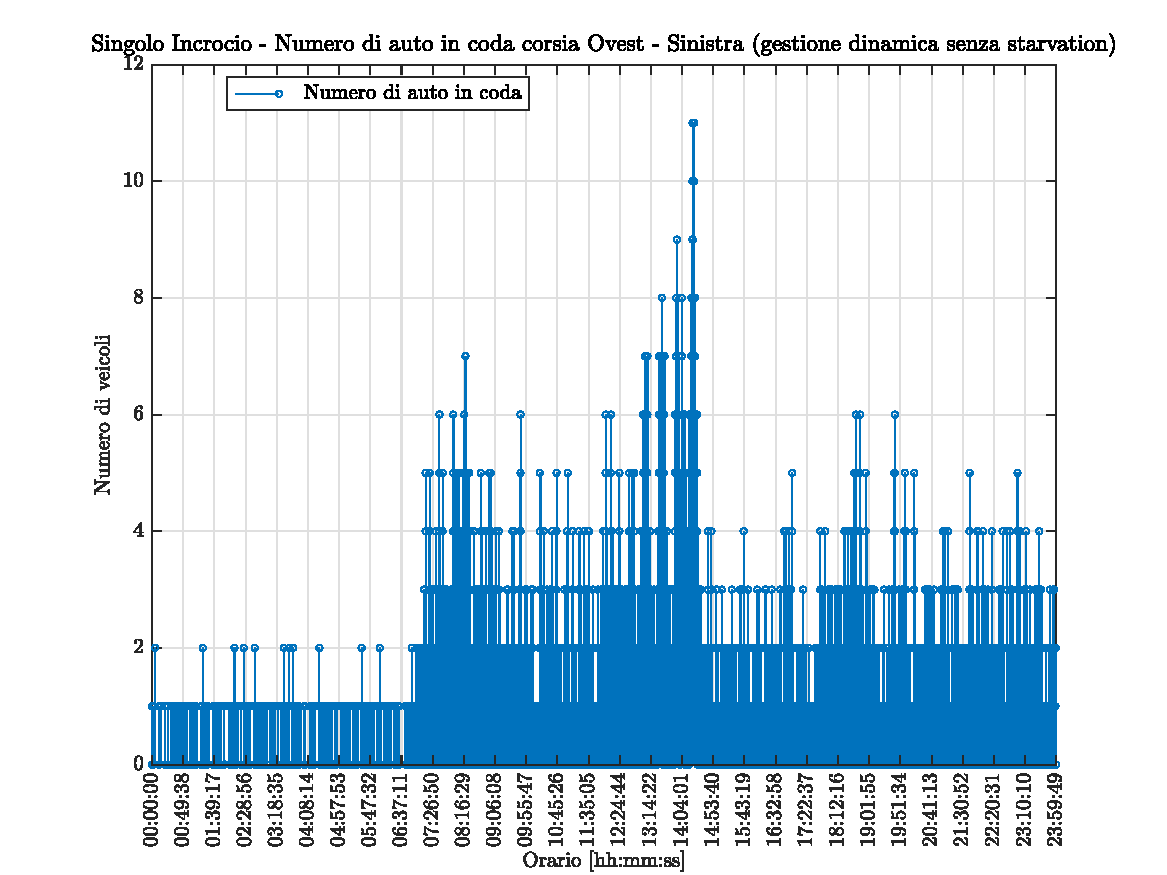
\includegraphics[width=0.9\textwidth]{figuraCodaGestioneDinamica.pdf}
  \caption{Numero di auto in coda in funzione dell'ora del giorno - Gestione dinamica del singolo incrocio senza starvation - $\mu$ casuali - corsia Ovest - Sinistra}
  \label{fig:}
\end{figure}
\begin{figure}[H]
\centering
  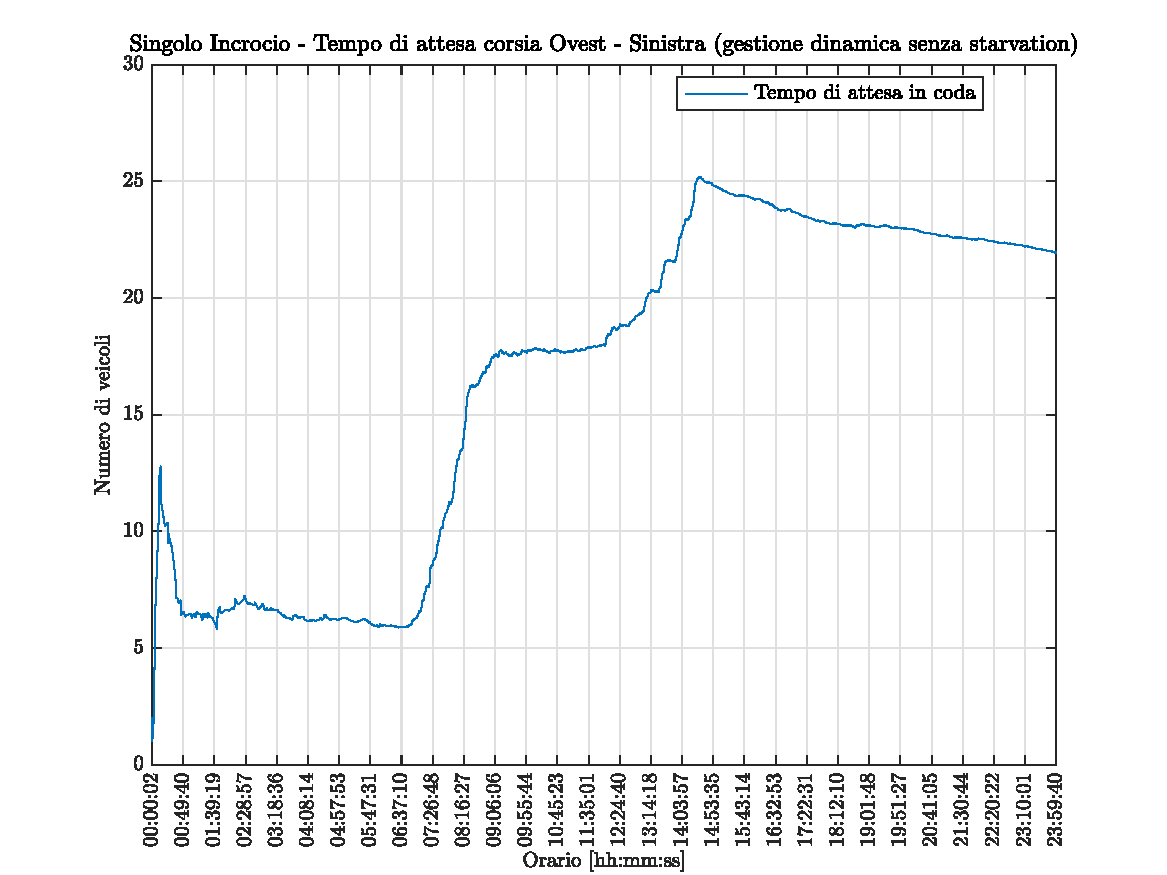
\includegraphics[width=0.9\textwidth]{figuraAttesaGestioneDinamica.pdf}
  \caption{Tempi di attesa in funzione dell'ora del giorno - Gestione dinamica del singolo incrocio senza starvation - $\mu$ casuali - corsia Ovest - Sinistra}
  \label{fig:}
\end{figure}
\newpage
\begin{figure}[H]
\centering
  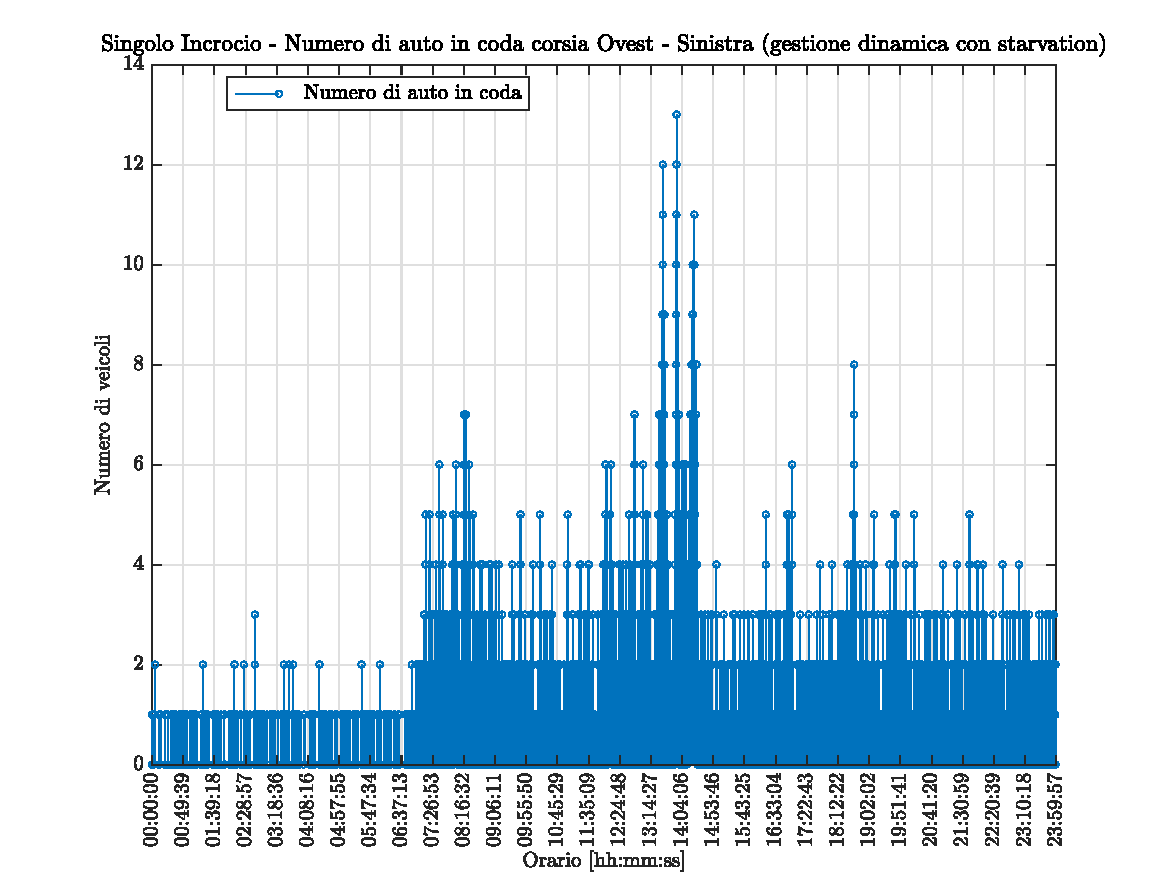
\includegraphics[width=0.9\textwidth]{figuraCodaGestioneDinamicaStarvation.pdf}
  \caption{Numero di auto in coda in funzione dell'ora del giorno - Gestione dinamica del singolo incrocio con starvation - $\mu$ casuali - corsia Ovest - Sinistra}
  \label{fig:}
\end{figure}
\begin{figure}[H]
\centering
  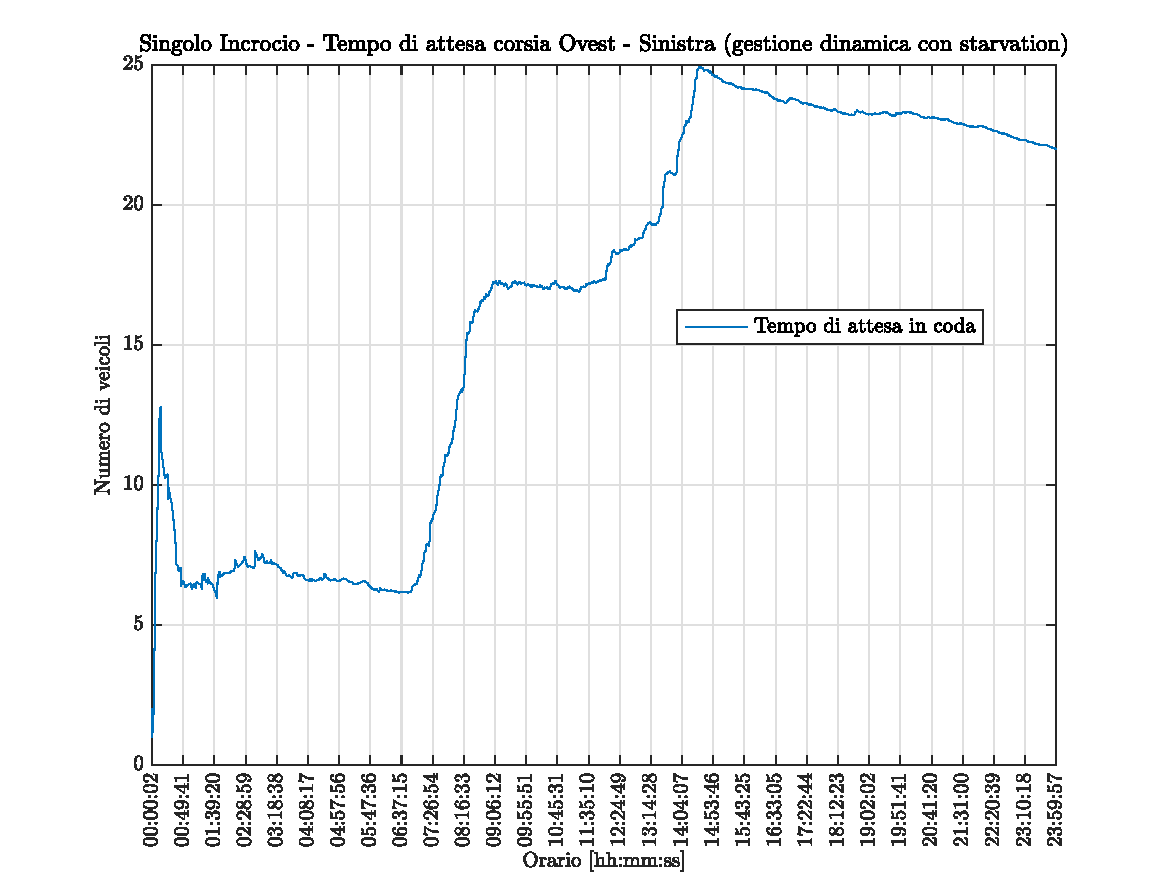
\includegraphics[width=0.9\textwidth]{figuraAttesaGestioneDinamicaStarvation.pdf}
  \caption{Tempi di attesa in funzione dell'ora del giorno - Gestione dinamica del singolo incrocio con starvation - $\mu$ casuali - corsia Ovest - Sinistra}
  \label{fig:}
\end{figure}
\newpage

Si può notare dalla tabella precedente e dai grafici riportati che per ogni situazione l'algoritmo di gestione dinamica applicato si comporta nettamente meglio di quello relativo ad una gestione statica, comunemente implementato, in una configurazione bilanciata, ovvero con un numero di auto totali che attraversano la giunzione paragonabile per ogni corsia. 

Nello specifico è interessante notare come vengano abbattuti drasticamente i tempi di attesa medi delle auto, e come nelle corsie più affollate anche il massimo numero di auto in coda raggiunto sia nettamente inferiore con la gestione proposta. Questo comporta innumerevoli benefici al traffico cittadino, meno congestionanto e quindi, di conseguenza, anche con meno emissioni di scarichi nocivi. 

Analizzando la corsia \textit{Ovest - Sinistra}, ovvero relativa alle auto che dal braccio ovest vogliono svoltare a sinistra, presa come esempio nella generazione dei grafici, in particolare, è facile comprendere che il massimo tempo di attesa raggiunto con la gestione statica sia di ben $80s$, a fronte dei $25s$ dei due algoritmi dinamici, così come è ben rilevabile che il massimo numero di auto in coda passi da 25 a 11 / 13.

Confrontando poi le gestioni con e senza \textit{starvation} si nota come le due siano essenzialmente equivalenti. Questo sia perché la gestione della \textit{starvation} interviene molto raramente, sia perché comunque, anche gestendo questa particolare variabile, l'algoritmo resta ottimizzato rispetto alla ricerca della corsia complementare a quella in attesa.

Queste considerazioni valgono per qualsiasi corsia, come emerge dalla tabella riportata, ed è da sottolineare che sono stati generati solo i grafici relativi ad una singola strada per praticità, mentre tutti i valori ottenuti sono stati fedelmente trascritti nella suddetta tabella.
\newline

Nella seguente simulazione ci si è concentrati sulla modellazione di una configurazione sbilanciata, con strade molto più affollate di altre, per comprendere anche in questo caso quanto sia pratico utilizzare un algoritmo di gestione dinamica. Nello specifico le corsie relative ai bracci \textit{Nord} e \textit{Sud} sono state volutamente congestionate, fissando il valore del parametro $\mu$ a 25, di base, a cui, si ricorda, deve essere sottratto un numero pari a 6 durante le ore di punta (mattina e pranzo) ed un numero pari a 3 durante l'ora di cena, mentre viene aggiunto un valore pari ad 80 durante la notte, per simulare il normale afflusso dei veicoli rispetto allo specifico periodo della giornata. Una spiegazione più approfondita di tutto ciò è stata già data nel \textit{Capitolo \ref{capitolo1}}. Le strade dei bracci \textit{Est} ed \textit{Ovest}, invece sono state lasciate abbastanza libere ($\mu$ pari a 60).




\begin{table}[H]
\centering
\begin{tabular}{|C{2cm}|C{1.65cm}|C{1.65cm}|C{1.65cm}|C{1.65cm}|C{1.65cm}|C{1.65cm}|}
  \hline
  \multicolumn{7}{|c|}{\large Seconda simulazione: prime quattro corsie} \\\hline\hline
  \multirow{7}{2cm}{\centering \textit{\footnotesize{Corsia Ovest \newline --- \newline Sinistra}}}
  & \multicolumn{2}{C{3.7cm}|}{\textbf{$\mu$}} 
  & \multicolumn{2}{C{3.7cm}|}{\textbf{\footnotesize{Tempo di arrivo medio}}} 
  & \multicolumn{2}{C{3.7cm}|}{\textbf{\footnotesize{Numero di auto totale}}} \\\cline{2-7}
  & \multicolumn{2}{C{3.7cm}|}{60} 
  & \multicolumn{2}{C{3.7cm}|}{$41.59s$} 
  & \multicolumn{2}{C{3.7cm}|}{1238} \\\cline{2-7}
  & \multicolumn{2}{C{3.7cm}|}{\footnotesize{\textbf{Gestione statica}}} 
  & \multicolumn{2}{C{3.7cm}|}{\footnotesize{\textbf{Gestione dinamica senza starvation}}} 
  & \multicolumn{2}{C{3.7cm}|}{\footnotesize{\textbf{Gestione dinamica con starvation}}} \\\cline{2-7}
  & \scriptsize{Max numero auto in coda}
  & \scriptsize{Tempo di attesa medio}
  & \scriptsize{Max numero auto in coda}
  & \scriptsize{Tempo di attesa medio}
  & \scriptsize{Max numero auto in coda}
  & \scriptsize{Tempo di attesa medio}\\\cline{2-7}
  & 7
  & $29.81s$
  & 5
  & $14.93s$
  & 5
  & $14.36s$\\\hline\hline
    \multirow{7}{2cm}{\centering \textit{\footnotesize{Corsia Ovest \newline --- \newline Dritto/Destra}}}
  & \multicolumn{2}{C{3.7cm}|}{\textbf{$\mu$}} 
  & \multicolumn{2}{C{3.7cm}|}{\textbf{\footnotesize{Tempo di arrivo medio}}} 
  & \multicolumn{2}{C{3.7cm}|}{\textbf{\footnotesize{Numero di auto totale}}} \\\cline{2-7}
  & \multicolumn{2}{C{3.7cm}|}{60} 
  & \multicolumn{2}{C{3.7cm}|}{$41.59s$} 
  & \multicolumn{2}{C{3.7cm}|}{1237} \\\cline{2-7}
  & \multicolumn{2}{C{3.7cm}|}{\footnotesize{\textbf{Gestione statica}}} 
  & \multicolumn{2}{C{3.7cm}|}{\footnotesize{\textbf{Gestione dinamica senza starvation}}} 
  & \multicolumn{2}{C{3.7cm}|}{\footnotesize{\textbf{Gestione dinamica con starvation}}} \\\cline{2-7}
  & \scriptsize{Max numero auto in coda}
  & \scriptsize{Tempo di attesa medio}
  & \scriptsize{Max numero auto in coda}
  & \scriptsize{Tempo di attesa medio}
  & \scriptsize{Max numero auto in coda}
  & \scriptsize{Tempo di attesa medio}\\\cline{2-7}
  & 6
  & $29.56s$
  & 5
  & $17.30s$
  & 5
  & $17.29s$\\\hline\hline
  \multirow{7}{2cm}{\centering \textit{\footnotesize{Corsia Nord \newline --- \newline Sinistra}}}
  & \multicolumn{2}{C{3.7cm}|}{\textbf{$\mu$}} 
  & \multicolumn{2}{C{3.7cm}|}{\textbf{\footnotesize{Tempo di arrivo medio}}} 
  & \multicolumn{2}{C{3.7cm}|}{\textbf{\footnotesize{Numero di auto totale}}} \\\cline{2-7}
  & \multicolumn{2}{C{3.7cm}|}{25} 
  & \multicolumn{2}{C{3.7cm}|}{$17.33s$} 
  & \multicolumn{2}{C{3.7cm}|}{2859} \\\cline{2-7}
  & \multicolumn{2}{C{3.7cm}|}{\footnotesize{\textbf{Gestione statica}}} 
  & \multicolumn{2}{C{3.7cm}|}{\footnotesize{\textbf{Gestione dinamica senza starvation}}} 
  & \multicolumn{2}{C{3.7cm}|}{\footnotesize{\textbf{Gestione dinamica con starvation}}} \\\cline{2-7}
  & \scriptsize{Max numero auto in coda}
  & \scriptsize{Tempo di attesa medio}
  & \scriptsize{Max numero auto in coda}
  & \scriptsize{Tempo di attesa medio}
  & \scriptsize{Max numero auto in coda}
  & \scriptsize{Tempo di attesa medio}\\\cline{2-7}
  & 17
  & $57.01s$
  & 7
  & $14.31s$
  & 7
  & $14.05s$\\\hline\hline
  \multirow{7}{2cm}{\centering \textit{\footnotesize{Corsia Nord \newline --- \newline Dritto/Destra}}}
  & \multicolumn{2}{C{3.7cm}|}{\textbf{$\mu$}} 
  & \multicolumn{2}{C{3.7cm}|}{\textbf{\footnotesize{Tempo di arrivo medio}}} 
  & \multicolumn{2}{C{3.7cm}|}{\textbf{\footnotesize{Numero di auto totale}}} \\\cline{2-7}
  & \multicolumn{2}{C{3.7cm}|}{25} 
  & \multicolumn{2}{C{3.7cm}|}{$17.33s$} 
  & \multicolumn{2}{C{3.7cm}|}{2872} \\\cline{2-7}
  & \multicolumn{2}{C{3.7cm}|}{\footnotesize{\textbf{Gestione statica}}} 
  & \multicolumn{2}{C{3.7cm}|}{\footnotesize{\textbf{Gestione dinamica senza starvation}}} 
  & \multicolumn{2}{C{3.7cm}|}{\footnotesize{\textbf{Gestione dinamica con starvation}}} \\\cline{2-7}
  & \scriptsize{Max numero auto in coda}
  & \scriptsize{Tempo di attesa medio}
  & \scriptsize{Max numero auto in coda}
  & \scriptsize{Tempo di attesa medio}
  & \scriptsize{Max numero auto in coda}
  & \scriptsize{Tempo di attesa medio}\\\cline{2-7}
  & 14
  & $51.36s$
  & 7
  & $12.83s$
  & 7
  & $13.18s$\\\hline
\end{tabular}
\caption{Tabella di comparazione fra algoritmi di gestione del singolo incrocio
- prime quattro corsie - configurazione sbilanciata}
\label{table:keytable}
\end{table}
\newpage

\begin{table}[H]
\centering
\begin{tabular}{|C{2cm}|C{1.65cm}|C{1.65cm}|C{1.65cm}|C{1.65cm}|C{1.65cm}|C{1.65cm}|}
  \hline
  \multicolumn{7}{|c|}{\large Seconda simulazione: ultime quattro corsie} \\\hline\hline
  \multirow{7}{2cm}{\centering \textit{\footnotesize{Corsia Est \newline --- \newline Sinistra}}}
  & \multicolumn{2}{C{3.7cm}|}{\textbf{$\mu$}} 
  & \multicolumn{2}{C{3.7cm}|}{\textbf{\footnotesize{Tempo di arrivo medio}}} 
  & \multicolumn{2}{C{3.7cm}|}{\textbf{\footnotesize{Numero di auto totale}}} \\\cline{2-7}
  & \multicolumn{2}{C{3.7cm}|}{60} 
  & \multicolumn{2}{C{3.7cm}|}{$41.59s$} 
  & \multicolumn{2}{C{3.7cm}|}{1226} \\\cline{2-7}
  & \multicolumn{2}{C{3.7cm}|}{\footnotesize{\textbf{Gestione statica}}} 
  & \multicolumn{2}{C{3.7cm}|}{\footnotesize{\textbf{Gestione dinamica senza starvation}}} 
  & \multicolumn{2}{C{3.7cm}|}{\footnotesize{\textbf{Gestione dinamica con starvation}}} \\\cline{2-7}
  & \scriptsize{Max numero auto in coda}
  & \scriptsize{Tempo di attesa medio}
  & \scriptsize{Max numero auto in coda}
  & \scriptsize{Tempo di attesa medio}
  & \scriptsize{Max numero auto in coda}
  & \scriptsize{Tempo di attesa medio}\\\cline{2-7}
  & 5
  & $32.61s$
  & 4
  & $17.11s$
  & 4
  & $17.74s$\\\hline\hline
    \multirow{7}{2cm}{\centering \textit{\footnotesize{Corsia Est \newline --- \newline Dritto/Destra}}}
  & \multicolumn{2}{C{3.7cm}|}{\textbf{$\mu$}} 
  & \multicolumn{2}{C{3.7cm}|}{\textbf{\footnotesize{Tempo di arrivo medio}}} 
  & \multicolumn{2}{C{3.7cm}|}{\textbf{\footnotesize{Numero di auto totale}}} \\\cline{2-7}
  & \multicolumn{2}{C{3.7cm}|}{60} 
  & \multicolumn{2}{C{3.7cm}|}{$41.59s$} 
  & \multicolumn{2}{C{3.7cm}|}{1254} \\\cline{2-7}
  & \multicolumn{2}{C{3.7cm}|}{\footnotesize{\textbf{Gestione statica}}} 
  & \multicolumn{2}{C{3.7cm}|}{\footnotesize{\textbf{Gestione dinamica senza starvation}}} 
  & \multicolumn{2}{C{3.7cm}|}{\footnotesize{\textbf{Gestione dinamica con starvation}}} \\\cline{2-7}
  & \scriptsize{Max numero auto in coda}
  & \scriptsize{Tempo di attesa medio}
  & \scriptsize{Max numero auto in coda}
  & \scriptsize{Tempo di attesa medio}
  & \scriptsize{Max numero auto in coda}
  & \scriptsize{Tempo di attesa medio}\\\cline{2-7}
  & 6
  & $33.42s$
  & 5
  & $21.91s$
  & 5
  & $21.05s$\\\hline\hline
  \multirow{7}{2cm}{\centering \textit{\footnotesize{Corsia Sud \newline --- \newline Sinistra}}}
  & \multicolumn{2}{C{3.7cm}|}{\textbf{$\mu$}} 
  & \multicolumn{2}{C{3.7cm}|}{\textbf{\footnotesize{Tempo di arrivo medio}}} 
  & \multicolumn{2}{C{3.7cm}|}{\textbf{\footnotesize{Numero di auto totale}}} \\\cline{2-7}
  & \multicolumn{2}{C{3.7cm}|}{25} 
  & \multicolumn{2}{C{3.7cm}|}{$17.33s$} 
  & \multicolumn{2}{C{3.7cm}|}{2875} \\\cline{2-7}
  & \multicolumn{2}{C{3.7cm}|}{\footnotesize{\textbf{Gestione statica}}} 
  & \multicolumn{2}{C{3.7cm}|}{\footnotesize{\textbf{Gestione dinamica senza starvation}}} 
  & \multicolumn{2}{C{3.7cm}|}{\footnotesize{\textbf{Gestione dinamica con starvation}}} \\\cline{2-7}
  & \scriptsize{Max numero auto in coda}
  & \scriptsize{Tempo di attesa medio}
  & \scriptsize{Max numero auto in coda}
  & \scriptsize{Tempo di attesa medio}
  & \scriptsize{Max numero auto in coda}
  & \scriptsize{Tempo di attesa medio}\\\cline{2-7}
  & 15
  & $53.73s$
  & 6
  & $17.69s$
  & 6
  & $17.86s$\\\hline\hline
  \multirow{7}{2cm}{\centering \textit{\footnotesize{Corsia Sud \newline --- \newline Dritto/Destra}}}
  & \multicolumn{2}{C{3.7cm}|}{\textbf{$\mu$}} 
  & \multicolumn{2}{C{3.7cm}|}{\textbf{\footnotesize{Tempo di arrivo medio}}} 
  & \multicolumn{2}{C{3.7cm}|}{\textbf{\footnotesize{Numero di auto totale}}} \\\cline{2-7}
  & \multicolumn{2}{C{3.7cm}|}{25} 
  & \multicolumn{2}{C{3.7cm}|}{$17.33s$} 
  & \multicolumn{2}{C{3.7cm}|}{2885} \\\cline{2-7}
  & \multicolumn{2}{C{3.7cm}|}{\footnotesize{\textbf{Gestione statica}}} 
  & \multicolumn{2}{C{3.7cm}|}{\footnotesize{\textbf{Gestione dinamica senza starvation}}} 
  & \multicolumn{2}{C{3.7cm}|}{\footnotesize{\textbf{Gestione dinamica con starvation}}} \\\cline{2-7}
  & \scriptsize{Max numero auto in coda}
  & \scriptsize{Tempo di attesa medio}
  & \scriptsize{Max numero auto in coda}
  & \scriptsize{Tempo di attesa medio}
  & \scriptsize{Max numero auto in coda}
  & \scriptsize{Tempo di attesa medio}\\\cline{2-7}
  & 20
  & $55.14s$
  & 6
  & $16.86s$
  & 8
  & $17.77s$\\\hline
\end{tabular}
\caption{Tabella di comparazione fra algoritmi di gestione del singolo incrocio
- ultime quattro corsie - configurazione sbilanciata}
\label{table:keytable}
\end{table}

Di seguito sono riportati alcuni grafici relativi alla corsia \textit{Ovest - Sinistra}, poco affollata, ed a quella \textit{Nord - Sinistra}, più congestionata.
\newpage
\begin{figure}[H]
\centering
  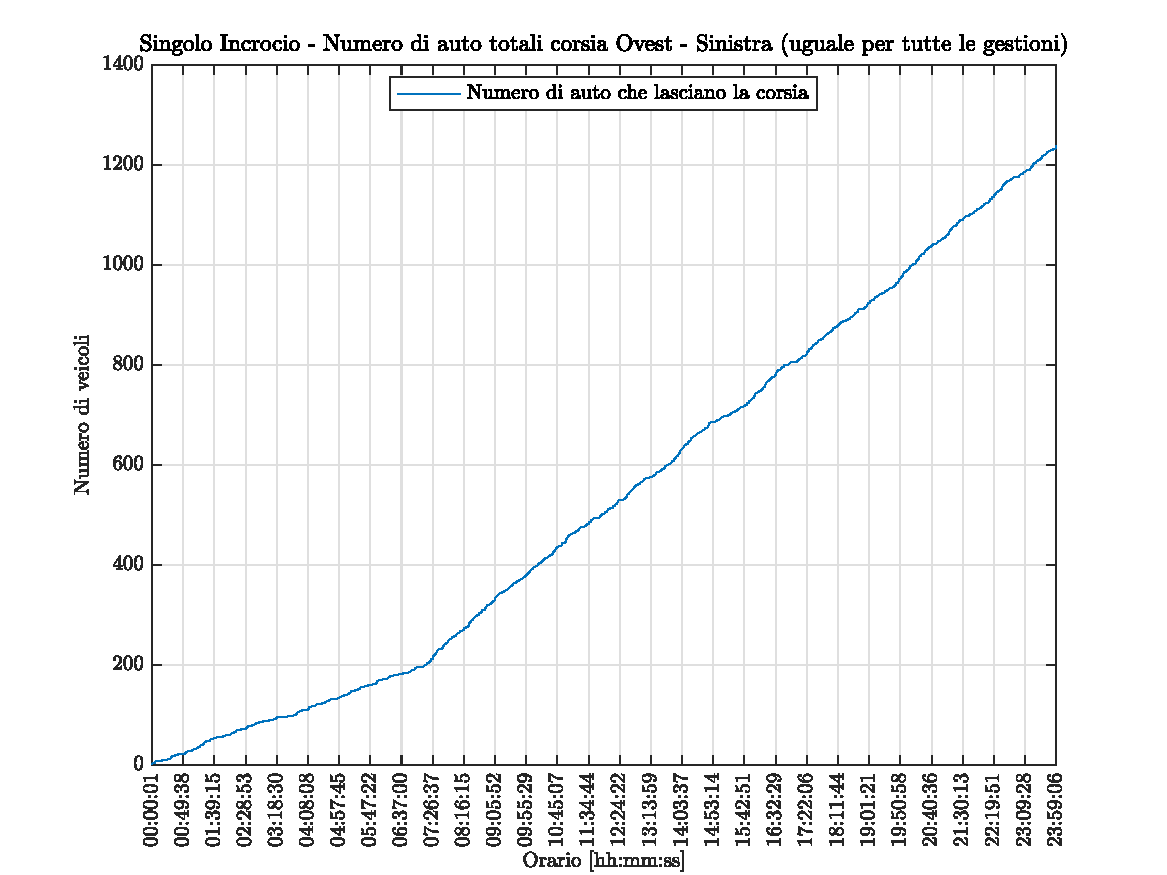
\includegraphics[width=0.9\textwidth]{figuraWestSinistraPartiti.pdf}
  \caption{Auto che hanno attraversato la corsia Ovest - Sinistra (uguale per i tre modelli di gestione) - configurazione sbilanciata}
  \label{fig:partitiMuSbil}
\end{figure}
\begin{figure}[H]
\centering
  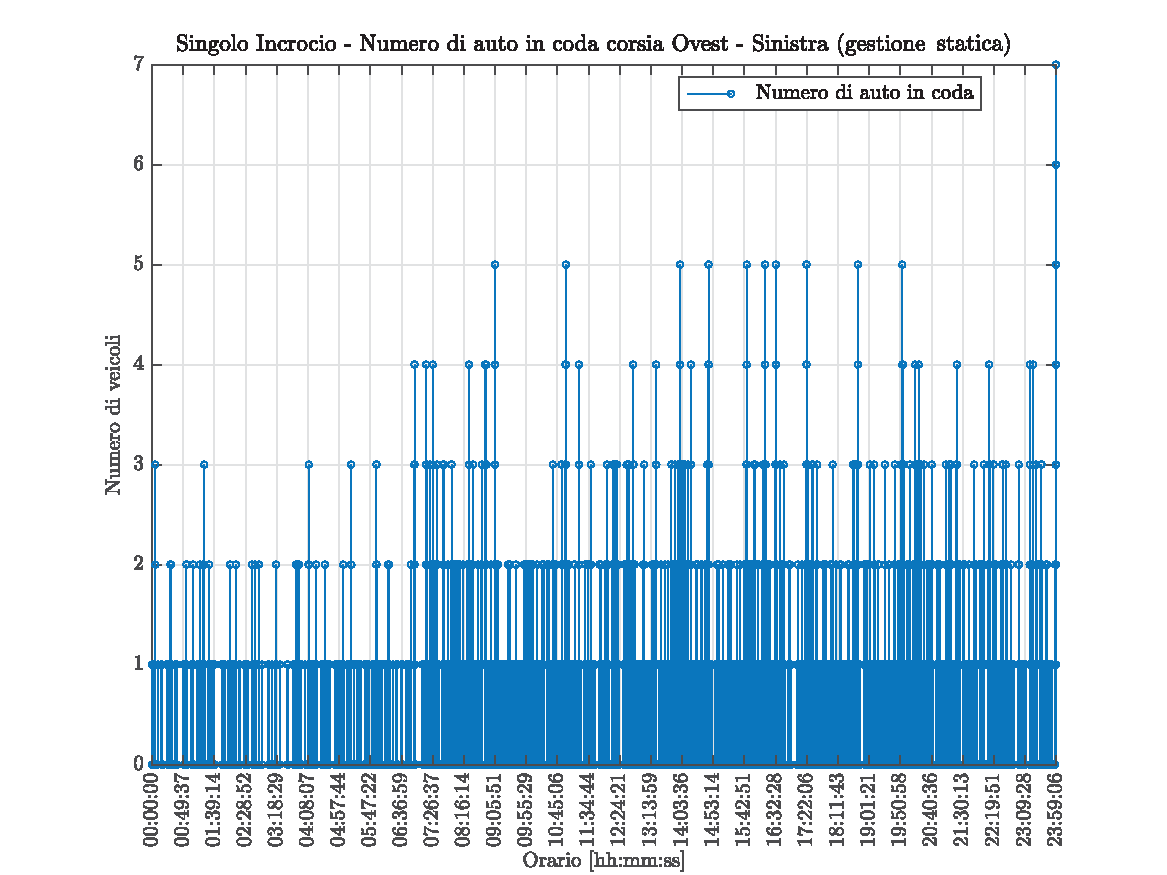
\includegraphics[width=0.9\textwidth]{figuraWestSinistraCodaGestioneStatica.pdf}
  \caption{Numero di auto in coda in funzione dell'ora del giorno - Gestione statica del singolo incrocio - Configurazione sbilanciata - corsia Ovest - Sinistra}
  \label{fig:}
\end{figure}

\newpage

\begin{figure}[H]
\centering
  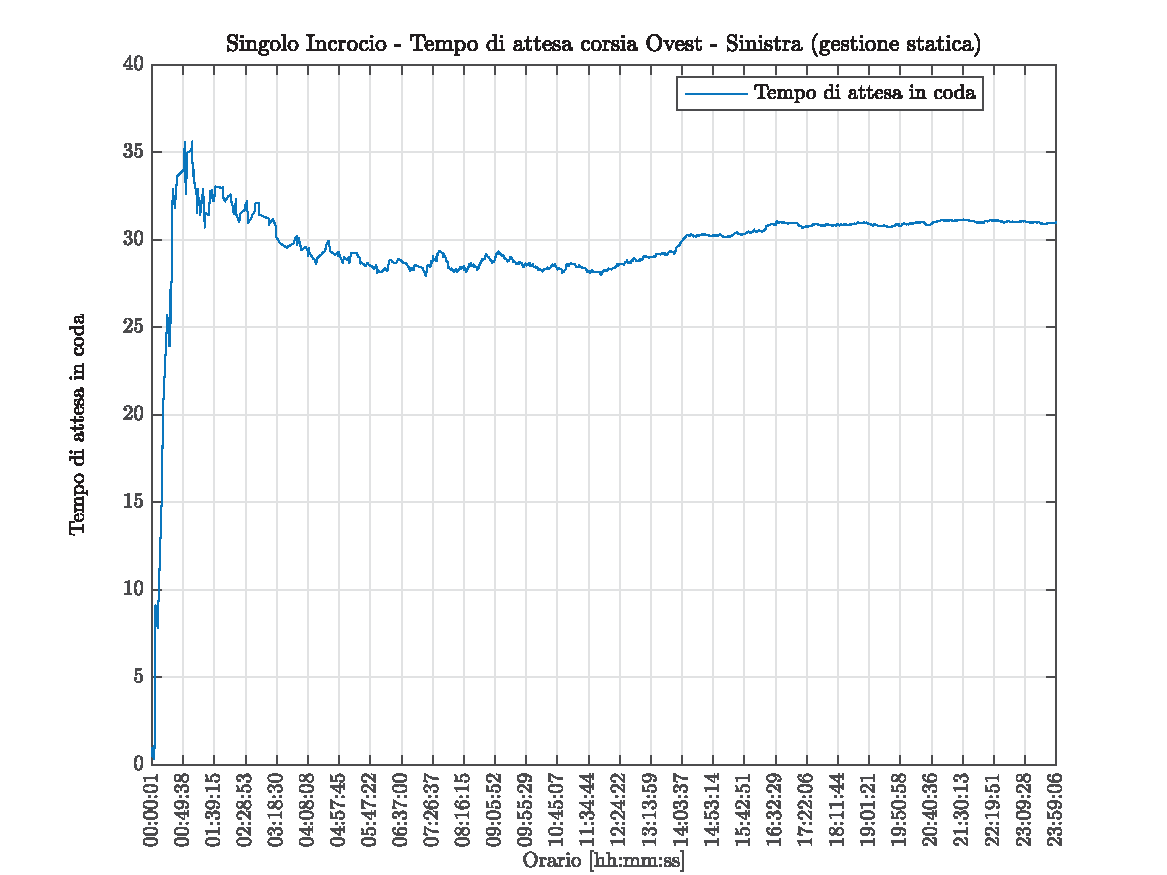
\includegraphics[width=0.9\textwidth]{figuraWestSinistraAttesaGestioneStatica.pdf}
  \caption{Tempi di attesa in funzione dell'ora del giorno - Gestione statica del singolo incrocio - Configurazione sbilanciata - corsia Ovest - Sinistra}
  \label{fig:}
\end{figure}
\begin{figure}[H]
\centering
  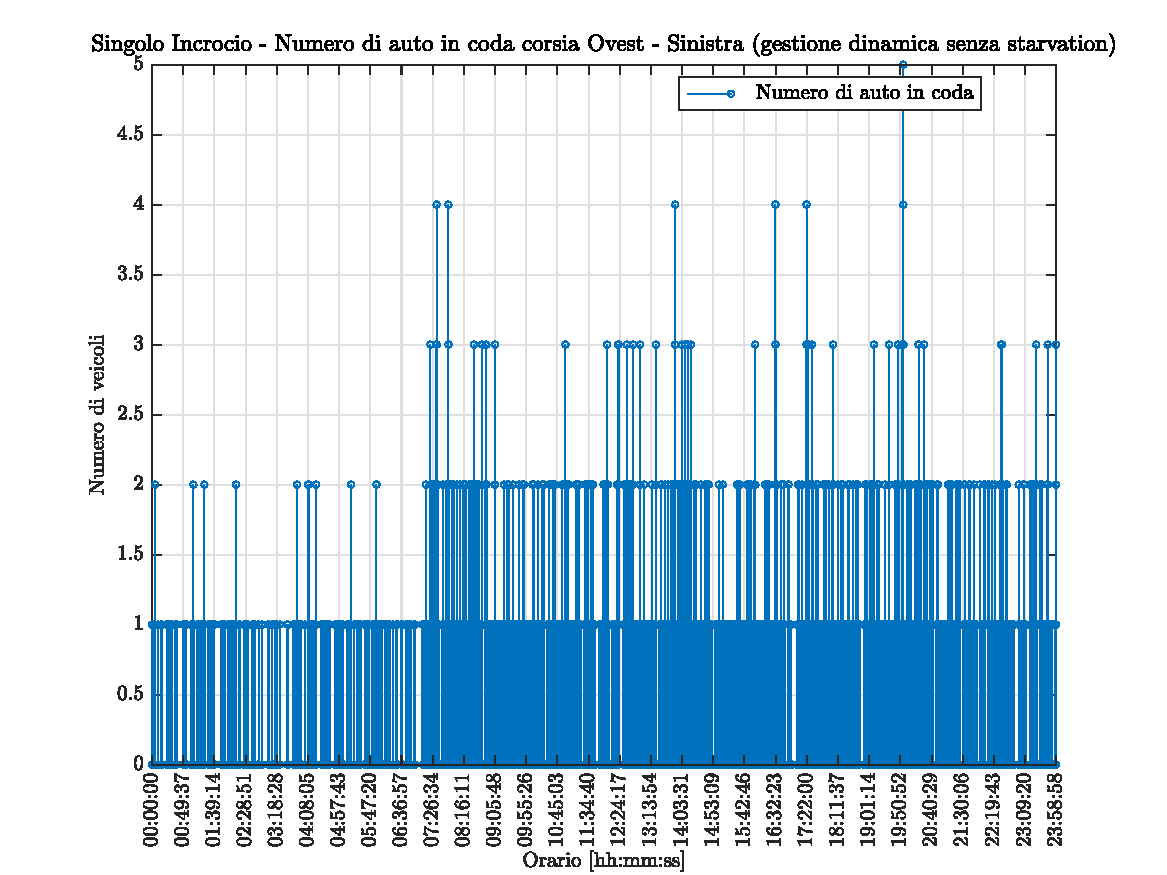
\includegraphics[width=0.9\textwidth]{figuraWestSinistraCodaGestioneDinamica.pdf}
  \caption{Numero di auto in coda in funzione dell'ora del giorno - Gestione dinamica del singolo incrocio senza starvation - Configurazione sbilanciata - corsia Ovest - Sinistra}
  \label{fig:}
\end{figure}

\newpage

\begin{figure}[H]
\centering
  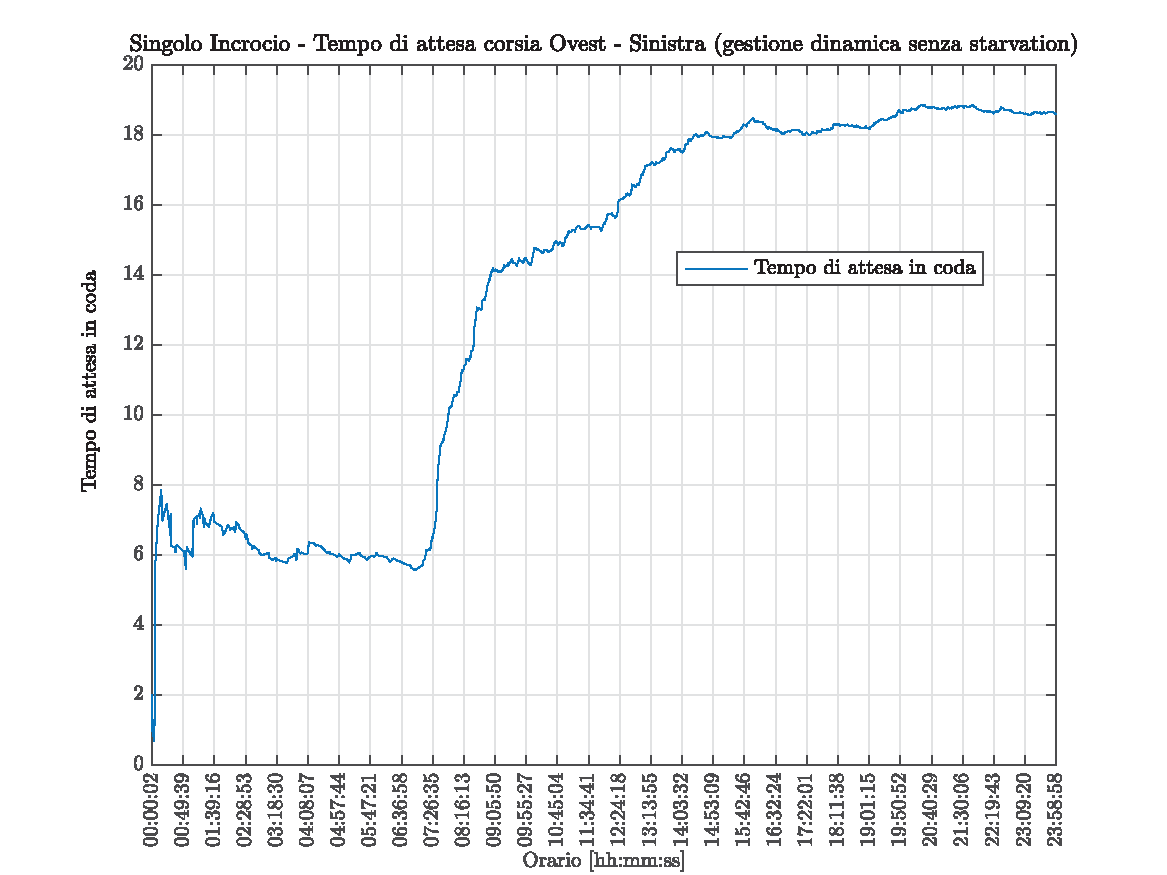
\includegraphics[width=0.9\textwidth]{figuraWestSinistraAttesaGestioneDinamica.pdf}
  \caption{Tempi di attesa in funzione dell'ora del giorno - Gestione dinamica del singolo incrocio senza starvation - Configurazione sbilanciata - corsia Ovest - Sinistra}
  \label{fig:}
\end{figure}
\begin{figure}[H]
\centering
  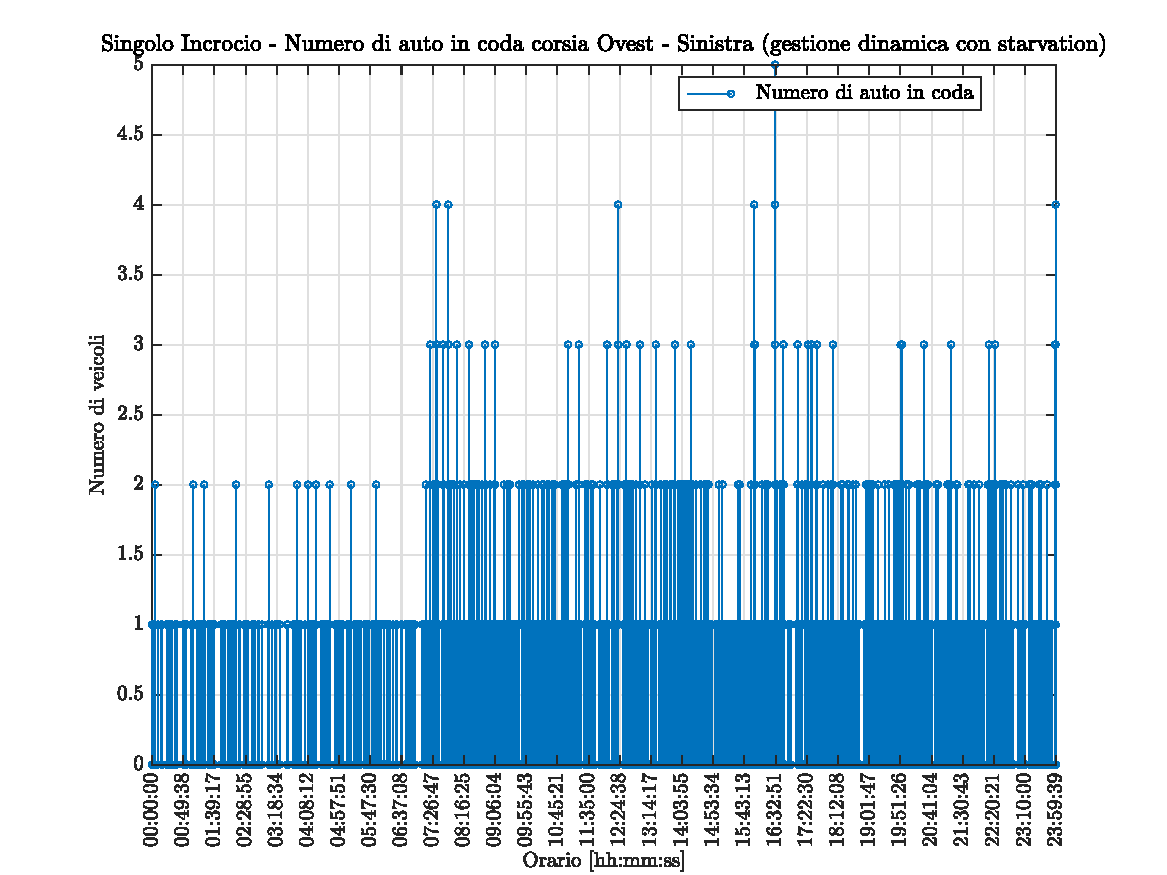
\includegraphics[width=0.9\textwidth]{figuraWestSinistraCodaGestioneDinamicaStarvation.pdf}
  \caption{Numero di auto in coda in funzione dell'ora del giorno - Gestione dinamica del singolo incrocio con starvation - Configurazione sbilanciata - corsia Ovest - Sinistra}
  \label{fig:}
\end{figure}
\newpage
\begin{figure}[H]
\centering
  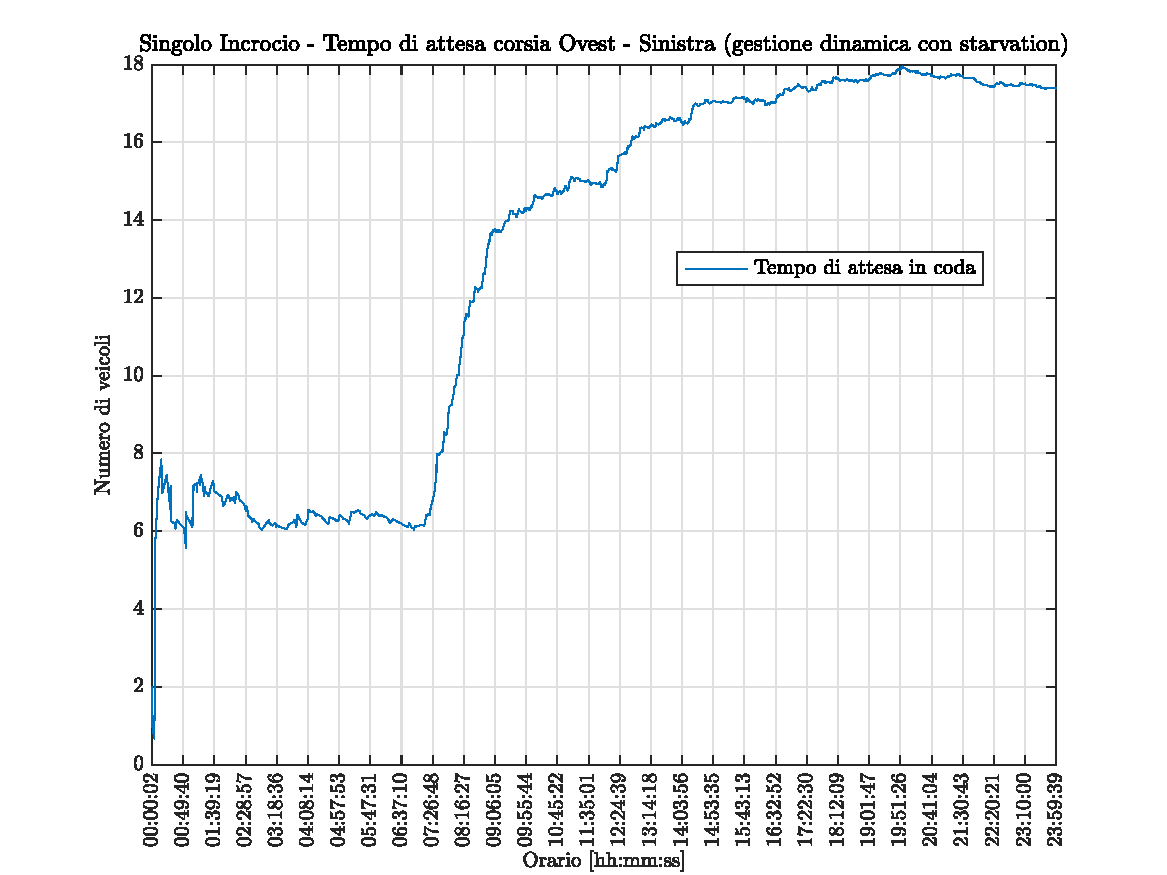
\includegraphics[width=0.9\textwidth]{figuraWestSinistraAttesaGestioneDinamicaStarvation.pdf}
  \caption{Tempi di attesa in funzione dell'ora del giorno - Gestione dinamica del singolo incrocio con starvation - Configurazione sbilanciata - corsia Ovest - Sinistra}
  \label{fig:}
\end{figure}

\newpage
\begin{figure}[H]
\centering
  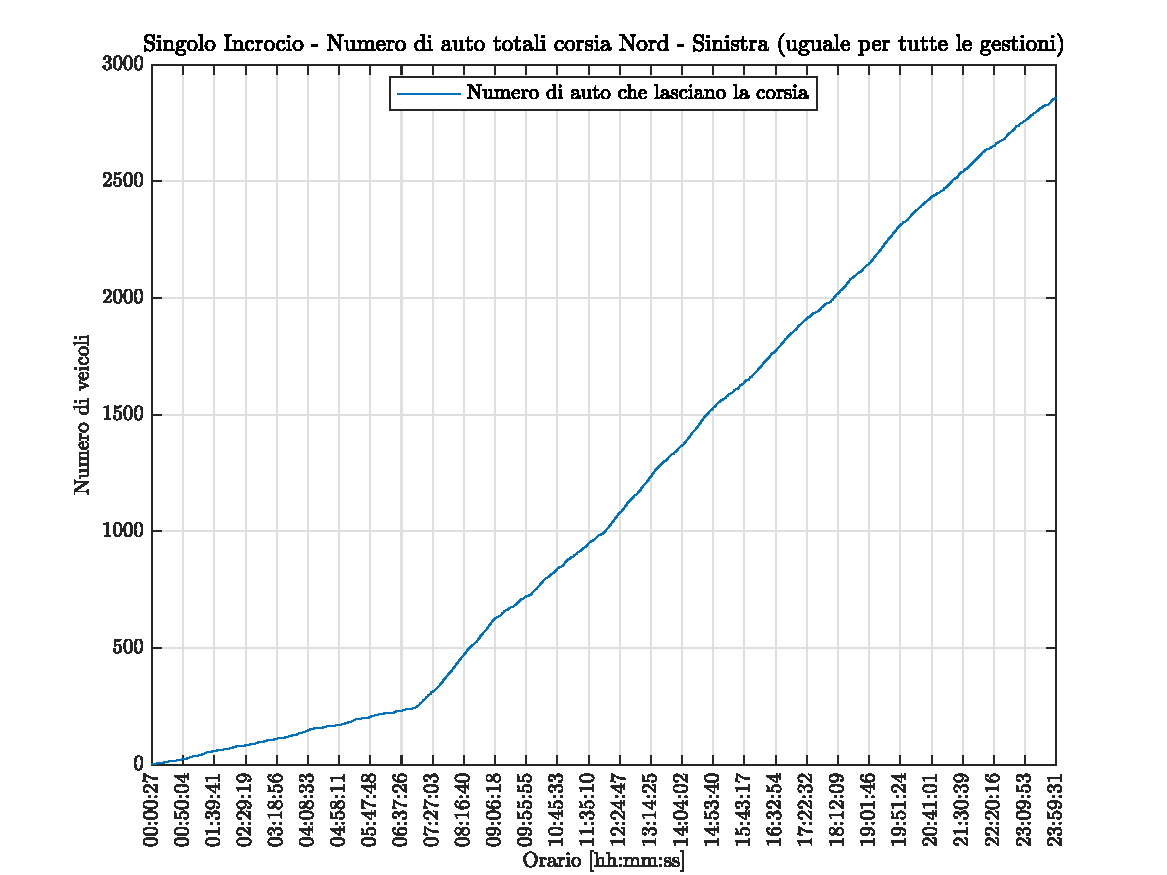
\includegraphics[width=0.9\textwidth]{figuraNordSinistraPartiti.pdf}
  \caption{Auto che hanno attraversato la corsia Nord - Sinistra (uguale per i tre modelli di gestione) - configurazione sbilanciata}
  \label{fig:partitiMuSbil}
\end{figure}
\begin{figure}[H]
\centering
  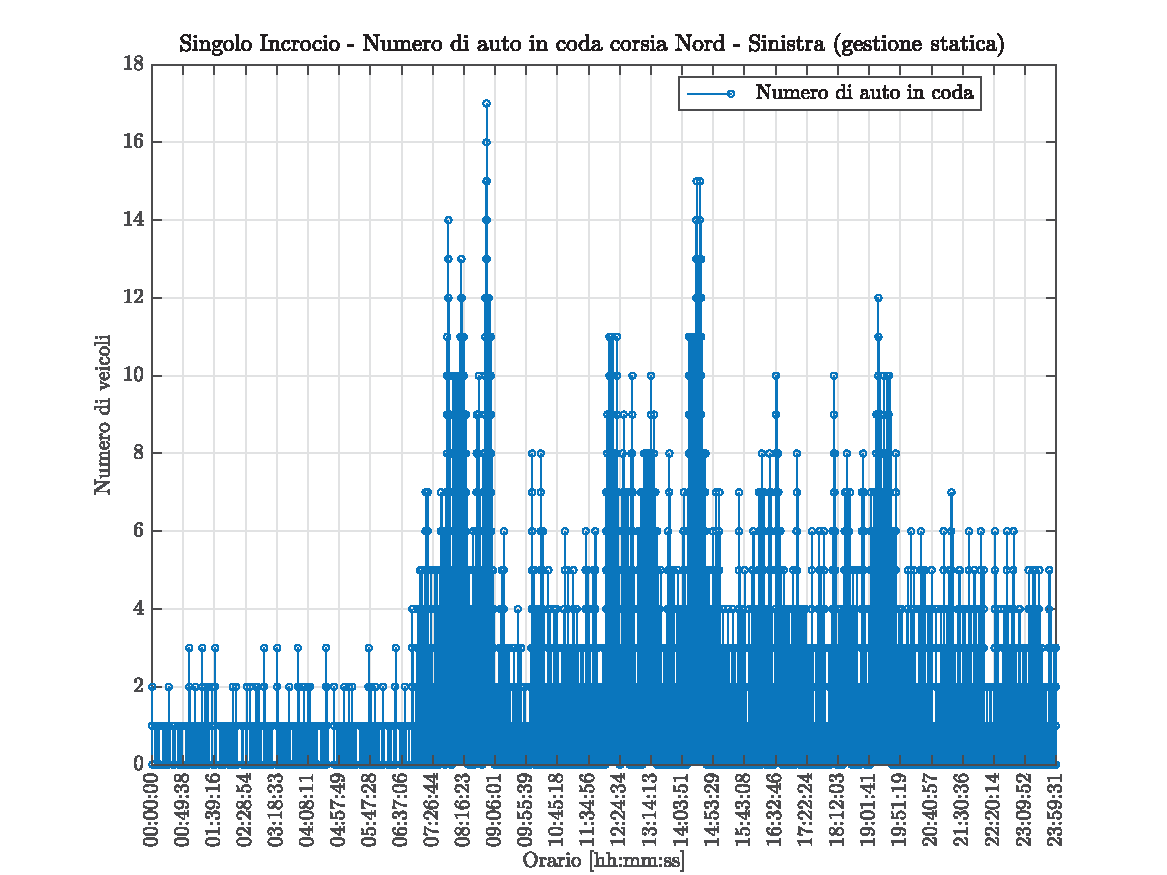
\includegraphics[width=0.9\textwidth]{figuraNordSinistraCodaGestioneStatica.pdf}
  \caption{Numero di auto in coda in funzione dell'ora del giorno - Gestione statica del singolo incrocio - Configurazione sbilanciata - corsia Nord - Sinistra}
  \label{fig:}
\end{figure}

\newpage

\begin{figure}[H]
\centering
  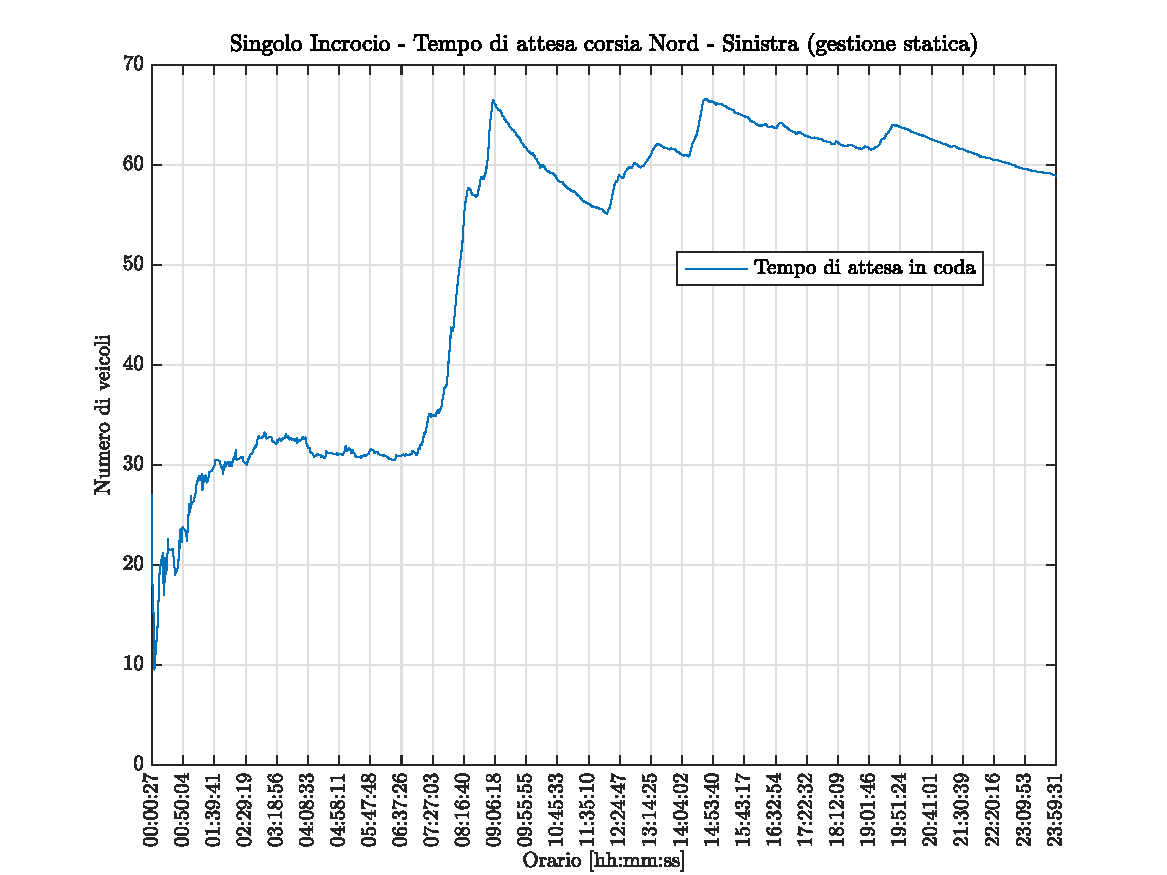
\includegraphics[width=0.9\textwidth]{figuraNordSinistraAttesaGestioneStatica.pdf}
  \caption{Tempi di attesa in funzione dell'ora del giorno - Gestione statica del singolo incrocio - Configurazione sbilanciata - corsia Nord - Sinistra}
  \label{fig:}
\end{figure}
\begin{figure}[H]
\centering
  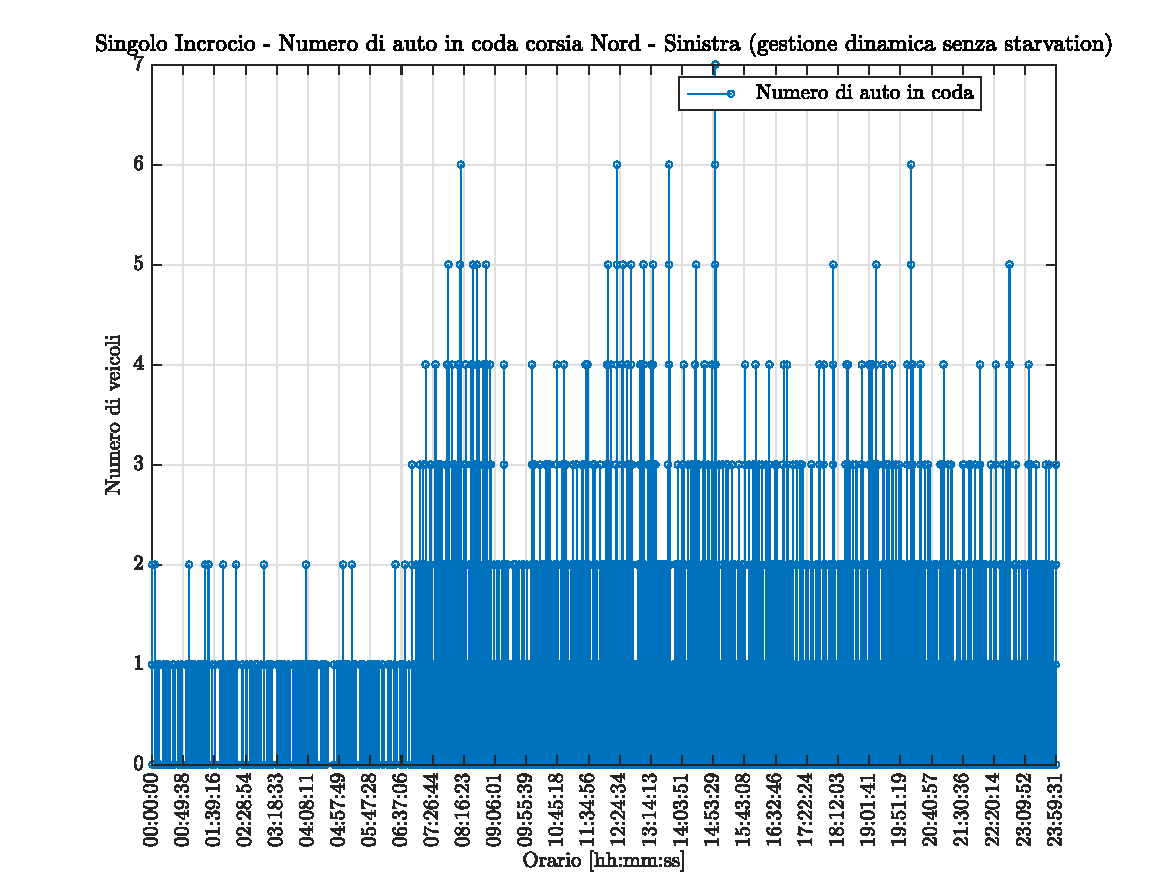
\includegraphics[width=0.9\textwidth]{figuraNordSinistraCodaGestioneDinamica.pdf}
  \caption{Numero di auto in coda in funzione dell'ora del giorno - Gestione dinamica del singolo incrocio senza starvation - Configurazione sbilanciata - corsia Nord - Sinistra}
  \label{fig:}
\end{figure}

\newpage

\begin{figure}[H]
\centering
  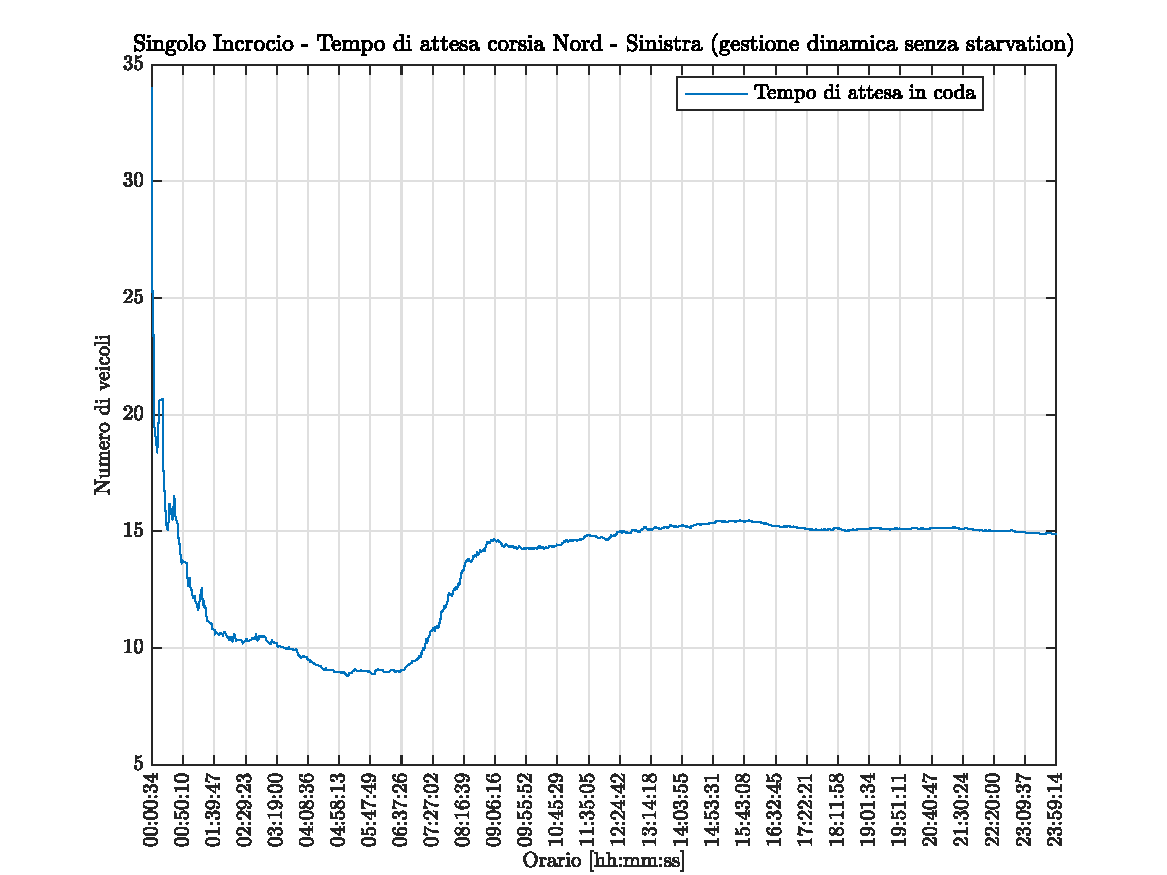
\includegraphics[width=0.9\textwidth]{figuraNordSinistraAttesaGestioneDinamica.pdf}
  \caption{Tempi di attesa in funzione dell'ora del giorno - Gestione dinamica del singolo incrocio senza starvation - Configurazione sbilanciata - corsia Nord - Sinistra}
  \label{fig:}
\end{figure}
\begin{figure}[H]
\centering
  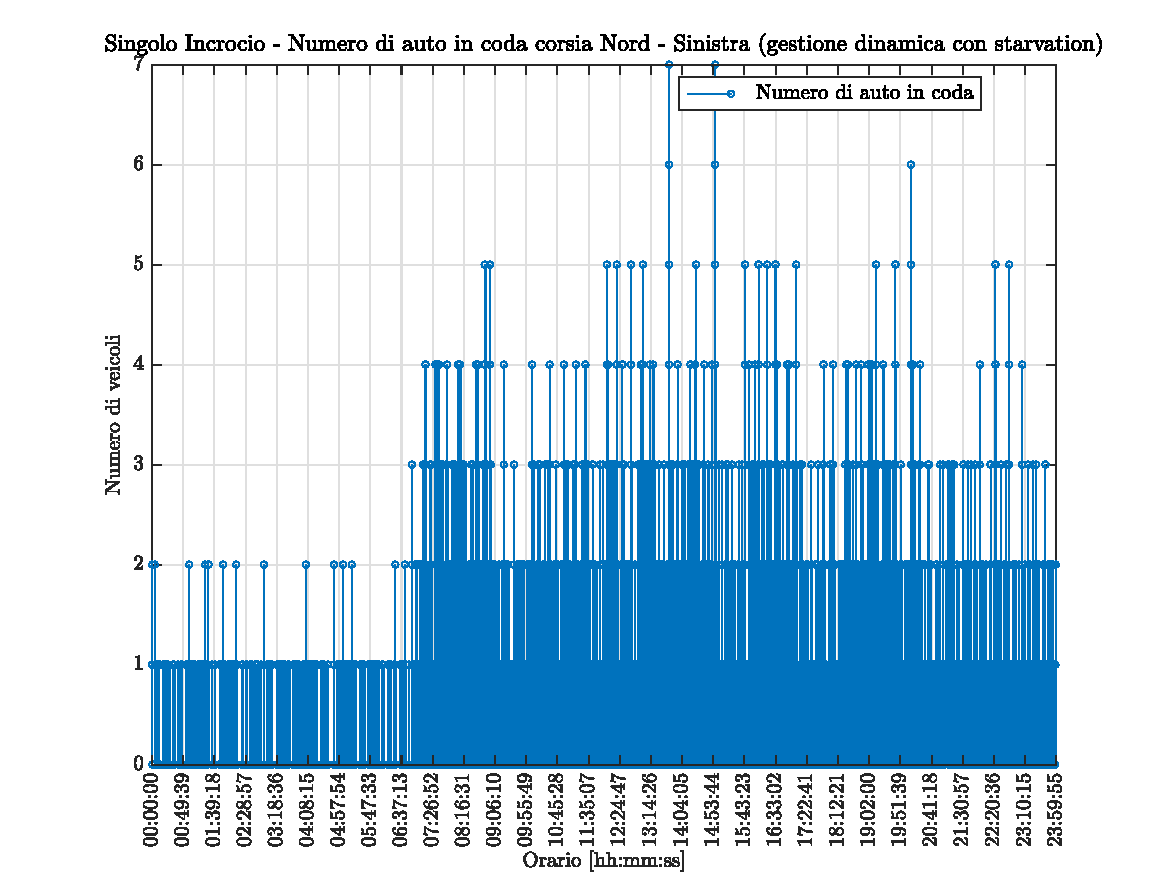
\includegraphics[width=0.9\textwidth]{figuraNordSinistraCodaGestioneDinamicaStarvation.pdf}
  \caption{Numero di auto in coda in funzione dell'ora del giorno - Gestione dinamica del singolo incrocio con starvation - Configurazione sbilanciata - corsia Nord - Sinistra}
  \label{fig:}
\end{figure}
\newpage
\begin{figure}[H]
\centering
  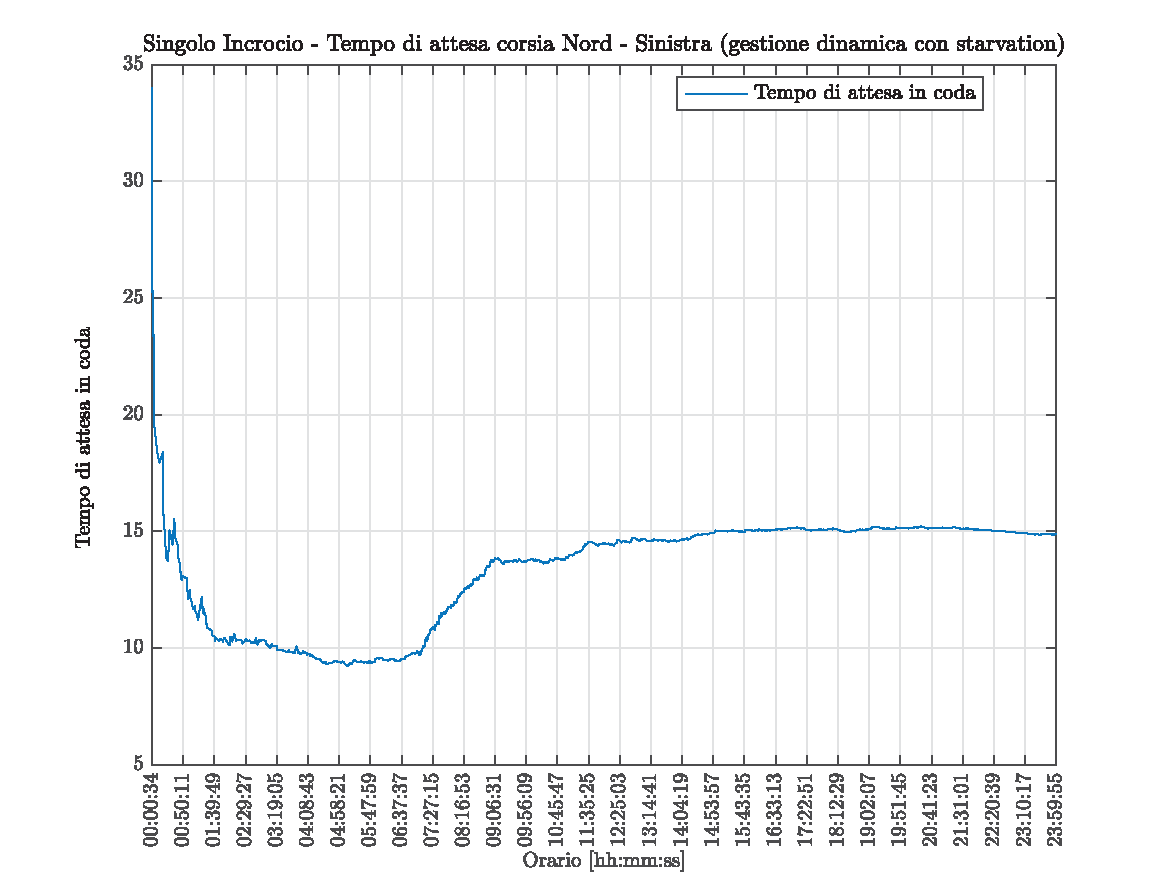
\includegraphics[width=0.9\textwidth]{figuraNordSinistraAttesaGestioneDinamicaStarvation.pdf}
  \caption{Tempi di attesa in funzione dell'ora del giorno - Gestione dinamica del singolo incrocio con starvation - Configurazione sbilanciata - corsia Nord - Sinistra}
  \label{fig:}
\end{figure}

Anche in questo caso si notano gli enormi benefici apportati da una gestione intelligente dell'incrocio, a seguito di un'implementazione di un algoritmo come quello proposto. In particolare appare chiaro come non solo vengano abbattuti i tempi di attesa, sia per le corsie affollate che per quelle con meno automobili, ma anche come questi vengano resi pressoché omogenei per tutte le corsie, e come l'ingorgo sia gestito egregiamente.

Per quanto concerne il numero massimo di auto in coda, si ha un sostanziale decremento per le strade più congestionate, mentre questo rimane stabile per quelle con meno entità, a fronte però di attese ridotte. Anche in questo caso la gestione della \textit{starvation} non penalizza lo smaltimento delle automobili.
\newline

In conclusione, dopo numerosi test svolti, si può affermare con certezza che l'algoritmo presentato sia funzionante e gestisca decisamente meglio gli incroci, in qualsiasi condizione, rispetto a quello tradizionale. Chiaramente bisogna considerare il fatto che si è esclusivamente analizzato il comportamento del codice presentato quando applicato ad una singola giunzione, quindi sorge spontanea la domanda: "cosa succederebbe se questo venisse applicato ad un cluster di incroci interconnessi fra loro? I benefici sarebbero altrettanto notevoli?". Per la risposta a questo legittimo interrogativo, nei prossimi capitoli verrà presentato un modello a 9 incroci interconnessi e comunicanti, basato su quanto già esposto, e sarà dimostrato come anche in una simulazione di questo genere sia indubbiamente conveniente gestire tali intersezioni dinamicamente.


























